\chapter{Protection implementation on Wishbone bus and test}
In the previous chapter, we conducted a comprehensive evaluation of fault injection attacks targeting three widely used on-chip bus protocols: Wishbone, AXI-Lite, and AXI. By examining their respective vulnerabilities in both control flow and data paths, we highlighted the architectural characteristics that influence their susceptibility to faults. Building upon those findings, this chapter focuses specifically on the Wishbone bus. We introduce a tailored countermeasure deployed within its critical transfer logic, and assess its effectiveness under the same fault model used earlier. Through comparative experiments and statistical analysis, we quantify the mitigation's impact on fault resilience and discuss the associated trade-offs, providing concrete insights for the design of more secure SoC communication architectures.
\section{Introduction of bus}

\section{Vulnerabilities exploitation on the Wishbone bus} 

We begin by analyzing the vulnerability associated with the \texttt{ACK} register. In Figure~\ref{nofault1}, the normal operation of the system is depicted, with the clock signal shown at the top. Following the initialization of variables by the \texttt{VerifyPin} routine, the CPU initiates a sequence of reads from the SRAM. The \texttt{ack1} signal, corresponding to SRAM, alternates between "$0$" and "$1$" on each clock cycle, whereas the other three \texttt{ACK} signals consistently remain low. The global data acknowledge signal, \texttt{ACK\_D}, is directly derived from \texttt{ack1} and is responsible for driving both address updates (\texttt{ADR}) and data sampling (\texttt{DAT}). As a result, both \texttt{ADR} and \texttt{DAT} signals are updated every two cycles.

During this operation, the CPU sequentially reads three values: 0x00000000, 0x04030201, and 0x00000000 from memory addresses 3, 4, and 5, respectively. The value stored at address 3 corresponds to the function code, while address 4 holds the card's PIN, and address 5 contains the user's PIN. Notably, the values retrieved from addresses 3 and 5 are identical. Each \texttt{DAT} value requires two clock cycles to reach the CPU and be committed into its cache. These values are subsequently stored into cache lines 3, 4, and 5.

Figure~\ref{fault1} illustrates the behavior under fault injection: a single bit-flip is introduced into \texttt{ack1} during the second cycle of period 2. This perturbation disturbs the expected timing of the data transfer. As highlighted in red, corrupted address and data values are observed in periods 2–3 and 3–4, respectively. Due to the fault, what was originally a two-cycle data transfer is now condensed into a single cycle. The cache mechanism reacts by reserving space prematurely, two cycles earlier than it should. Consequently, the third cache line incorrectly records 0x00000a8c at period 4 instead of the correct 0x00000000, while the fourth line, meant to store the card’s PIN, wrongly contains 0x00000000 at period 5 instead of the expected 0x04030201. These anomalies result in a flawed comparison: the program ends up verifying two identical user PINs, ultimately permitting unauthorized access.

At the RTL (Register Transfer Level), a single transient fault can lead to multiple bit-flips. Even if only one bit is initially targeted, the resulting effect may propagate, corrupting up to 64 bits within a register. From an instruction-level perspective, this can cause instruction repetition or skipping. Nonetheless, most operations such as \texttt{add}, \texttt{sub}, \texttt{and}, and \texttt{or} are idempotent—re-executing them has no net effect. As a result, such faults can often be leveraged to reliably skip instructions without unintended side effects from preceding operations.

\begin{figure}[t!]
  \centering
  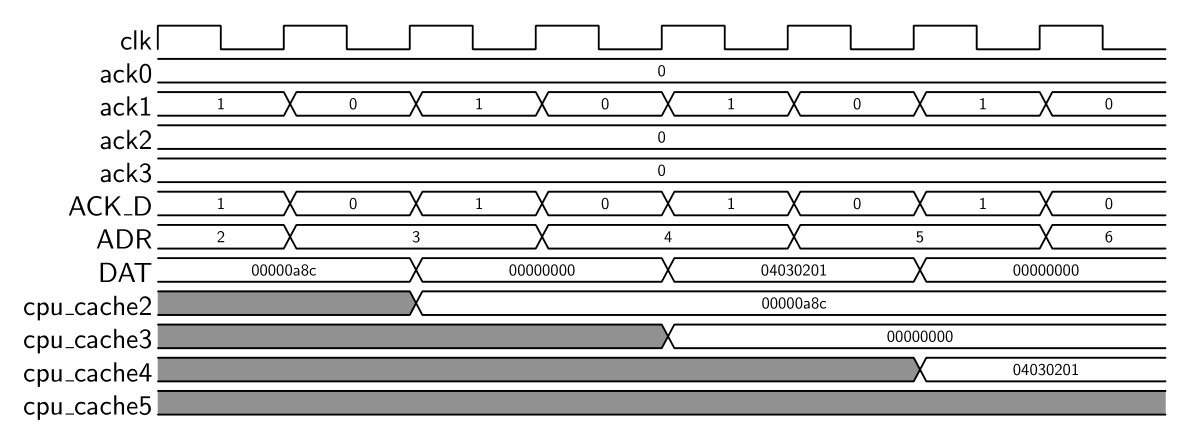
\includegraphics[width=\linewidth]{Chapitre4/figures/nofault1.png}
  \caption{Impact of acknowledge signal on address, data signals and CPU cache without attack}
  \label{nofault1}
\end{figure}

\begin{figure}[t!]
  \centering
  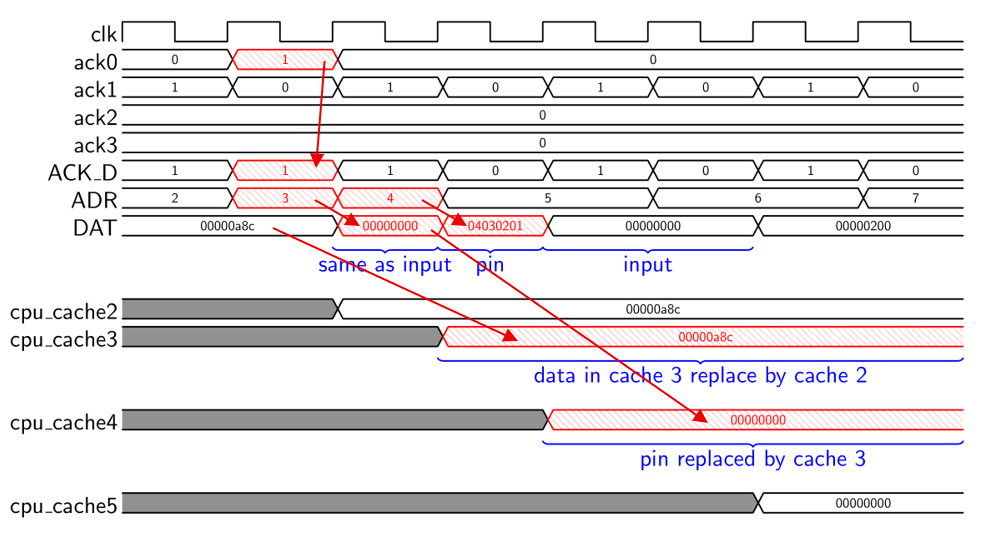
\includegraphics[width=\linewidth]{Chapitre4/figures/fault1.png}
  \caption{Impact of acknowledge signal on address, data signals and CPU cache with attack}
  \label{fault1}
\end{figure}

Next, we examine the impact of faults on the \texttt{grant} register. Figure~\ref{nofault2} depicts the expected behavior under normal operating conditions, with the clock waveform shown at the top. Initially, the \texttt{grant} register is set to 0, causing the CPU to fetch instruction values from the ROM. Starting from the second period, once the \texttt{grant} signal transitions to 1, the CPU begins accessing variable data stored in SRAM. The \texttt{ack1} signal, representing data acknowledge from the SRAM, alternates between "$0$" and "$1$" on each clock cycle, while the remaining \texttt{ACK} lines remain at "$0$". The global acknowledge signal \texttt{ACK\_D}, derived from \texttt{ack1}, orchestrates both the address increment (\texttt{ADR}) and data sampling (\texttt{DAT}), resulting in address and data updates occurring every two cycles.

During this process, the CPU retrieves the following sequence of data: 0x00000000, 0x04000000, and 0x10000018, located at addresses 0x7f0, 0x7f1, and 0x7f2, respectively. The content at 0x7f0 serves as the function code, while the first two bits at address 0x7f1 encode the size value, which is shared by both the card PIN and user PIN. The final value at 0x7f2 indicates the memory address pointing to the user's PIN. As in the previous case, each \texttt{DAT} value takes two cycles to propagate and is subsequently stored in cache addresses 0x1008, 0x1009, and 0x1010.

Figure~\ref{fault2} illustrates the behavior following a fault injection. A bit-flip is simultaneously introduced into both \texttt{ack0} and the \texttt{grant} register. The premature transition of \texttt{grant} causes the CPU to interpret control signals one cycle earlier than intended. Consequently, the acknowledge, address, and data signals all advance by one cycle. As in the previous scenario, this temporal shift in the \texttt{ACK} signal disrupts the timing of data reads. The third cache line mistakenly stores 0x0007c783 at cycle 3 in place of the correct 0x00000000, while the fourth cache line—intended to store the card PIN—incorrectly holds 0x00000000 instead of 0x04000000 at cycle 4. This leads to incorrect interpretation of the size value as zero, causing the loop body to execute zero times and thereby bypassing the authentication routine.

At the Register Transfer Level (RTL), a fault affecting the \texttt{grant} register may induce multiple bit-flips within the same cycle. From the perspective of instruction-level execution, such a fault can cause either premature or delayed signal responses. However, our current experimental observations indicate that faults targeting the \texttt{grant} register affect too many signals simultaneously, making it difficult to achieve precise fault effects. As such, isolated faults on \texttt{grant} have not yet resulted in successful exploitation within our current setup.

\begin{figure}[t!]
  \centering
  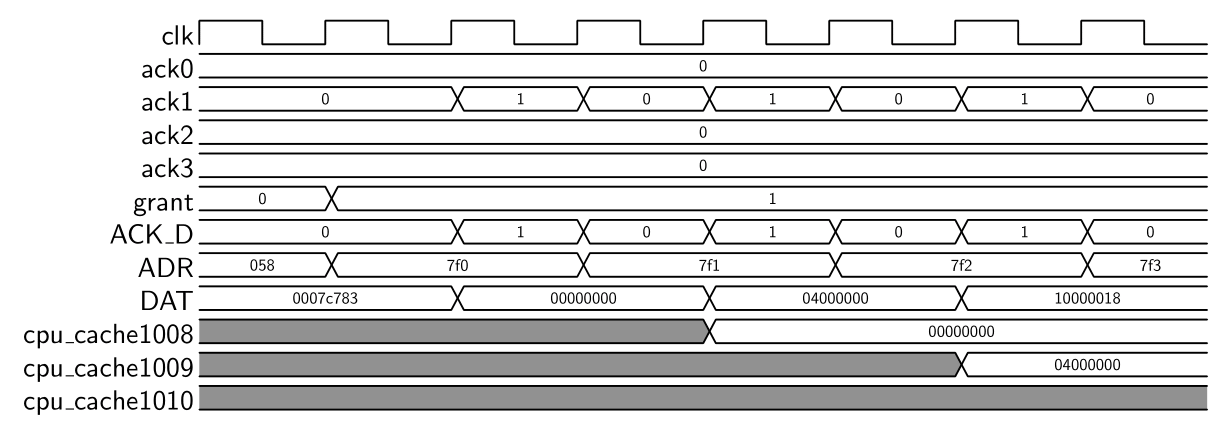
\includegraphics[width=\linewidth]{Chapitre4/figures/nofault2.png}
  \caption{Impact of grant signal on address, data signals and CPU cache without attack}
  \label{nofault2}
\end{figure}

\begin{figure}[t!]
  \centering
  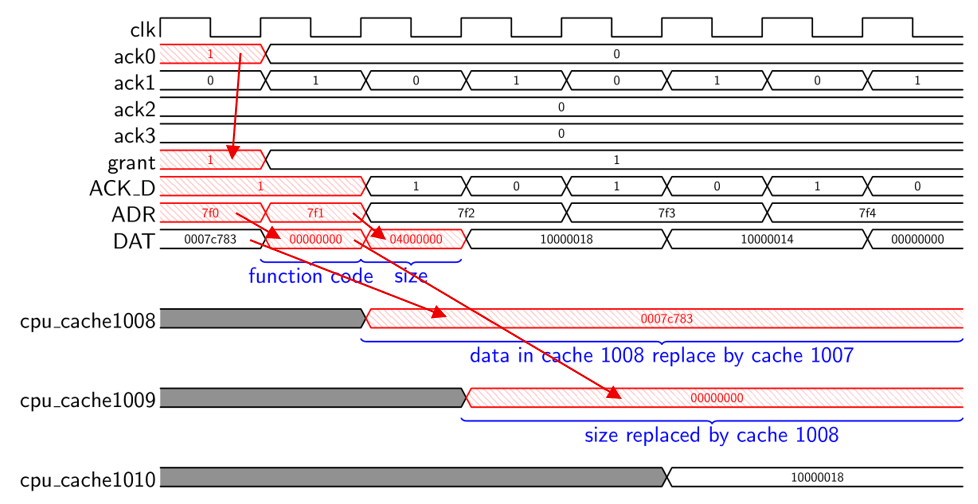
\includegraphics[width=\linewidth]{Chapitre4/figures/fault2.png}
  \caption{Impact of grant signal on address, data signals and CPU cache with attack}
  \label{fault2}
\end{figure}


The \texttt{SEL} register is vulnerable to various forms of fault injection. In the first attack scenario, referred to as data reset, the fault targets the data bus by manipulating the \texttt{SEL} signal. Under normal conditions—identical to those used in the \texttt{ACK} fault scenario—the CPU reads data from the SRAM, and the \texttt{SEL} register holds the value "0010". Each bit of the \texttt{SEL} signal is expanded to a 32-bit mask and then ANDed with the corresponding word in memory. In this case, the active selection results in SRAM data being masked with 0xffffffff, allowing the correct data to be transferred to the data bus.

However, if a fault occurs during the fifth cycle that forces the \texttt{SEL} register to "0000", each bit of the selection signal expands to 0x00000000. When ANDed with the corresponding memory data, this results in all selected words being zeroed. The four resulting 32-bit values (all 0x00000000) are then combined using a bitwise OR operation, yielding a final data word of 0x00000000. This corrupted value is then stored into the CPU cache.

When this fault takes place during the card PIN retrieval phase, the CPU ends up caching an all-zero value. If the user-provided PIN is also "0000", the comparison succeeds, resulting in unauthorized authentication. Notably, this attack achieves its effect by simultaneously resetting multiple bits of the \texttt{SEL} register, thereby masking the true contents of the data bus.

\begin{figure}[t!]
  \centering
  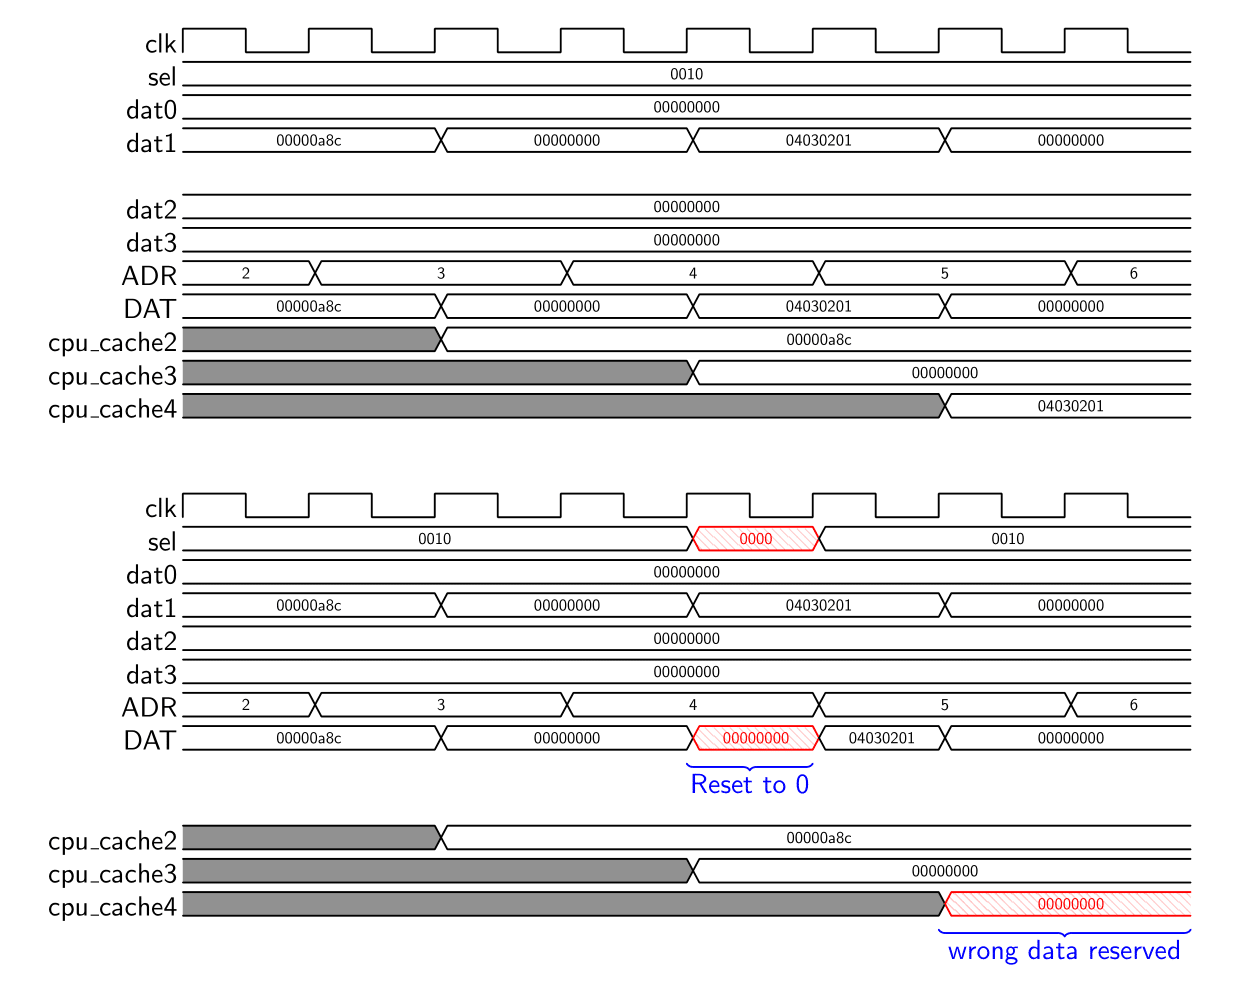
\includegraphics[width=\linewidth]{Chapitre4/figures/fault3.png}
  \caption{Impact of data reset on selection signal, data signals and CPU cache with/without attack}
  \label{fault3}
\end{figure}

In the second scenario, if a single unintended bit in the \texttt{SEL} register is set to "1" and the intended one is set to "0", this is called data misread. In our example as Figure \ref{fault4}, unlike SRAM is read in CPU in normal condition, ROM is read beacause of the attack on \texttt{SEL} register. In this case, the data "00000000" replace the correct card pin "04030201", cause the success.

\begin{figure}[t!]
  \centering
  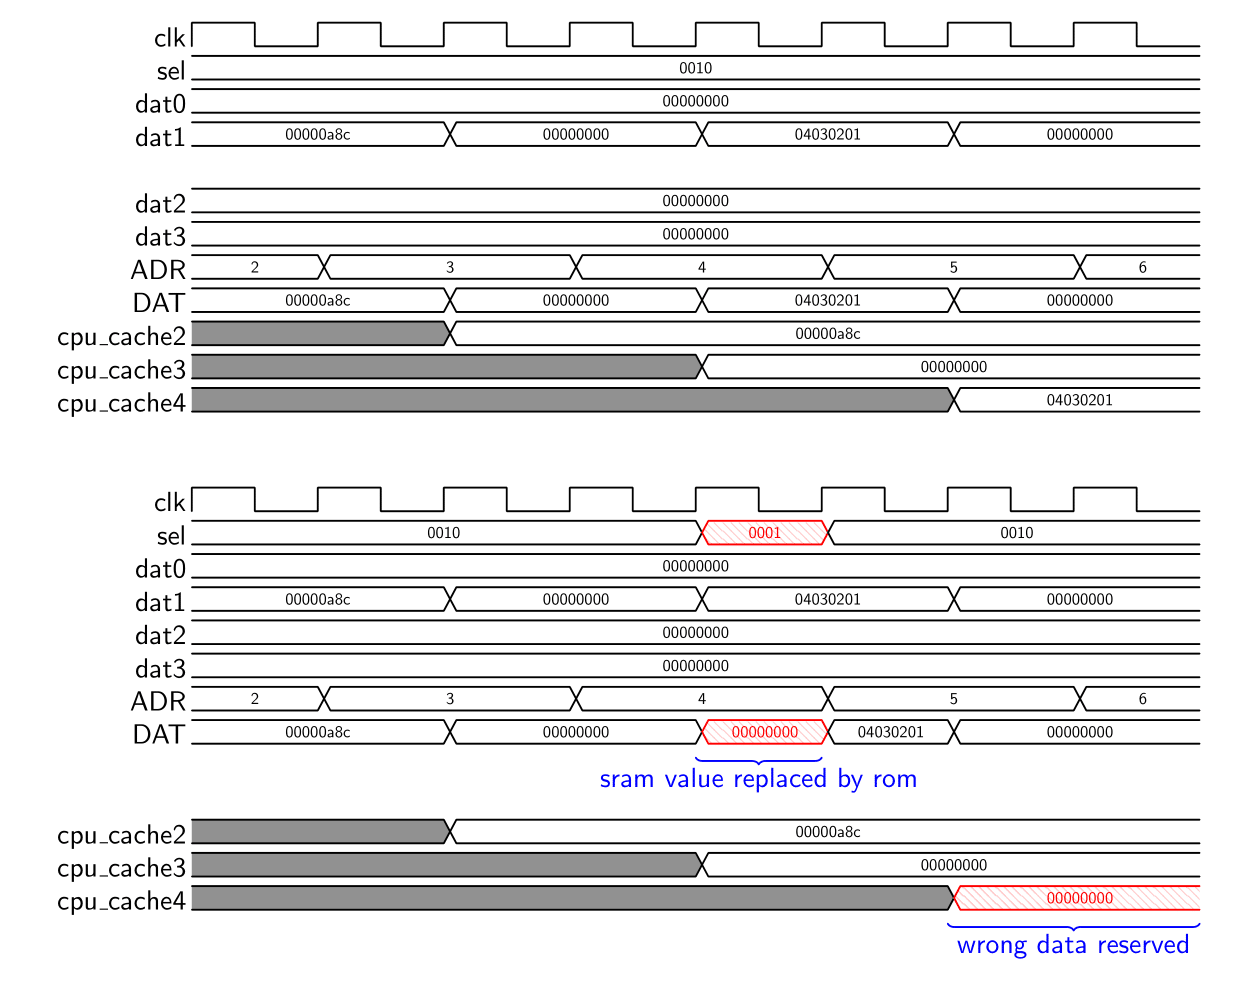
\includegraphics[width=\linewidth]{Chapitre4/figures/fault4.png}
  \caption{Impact of data misread on selection signal, data signals and CPU cache with/without attack}
  \label{fault4}
\end{figure}

In the third scenario, a fault causes more than one unintended bit in the \texttt{SEL} register to be set to "1", a condition referred to as data multiread. As shown in Figure~\ref{fault5}, the injected fault modifies \texttt{SEL} to "1100", resulting in both CSR and \texttt{MAIN\_RAM} being read by the CPU simultaneously. Since both memory regions were initialized with zero values, the data output from each is 0x00000000. The resulting \texttt{DAT} signal transmitted to the CPU is the bitwise OR of the two, which remains 0x00000000. This leads to a successful authentication bypass.

\begin{figure}[t!]
  \centering
  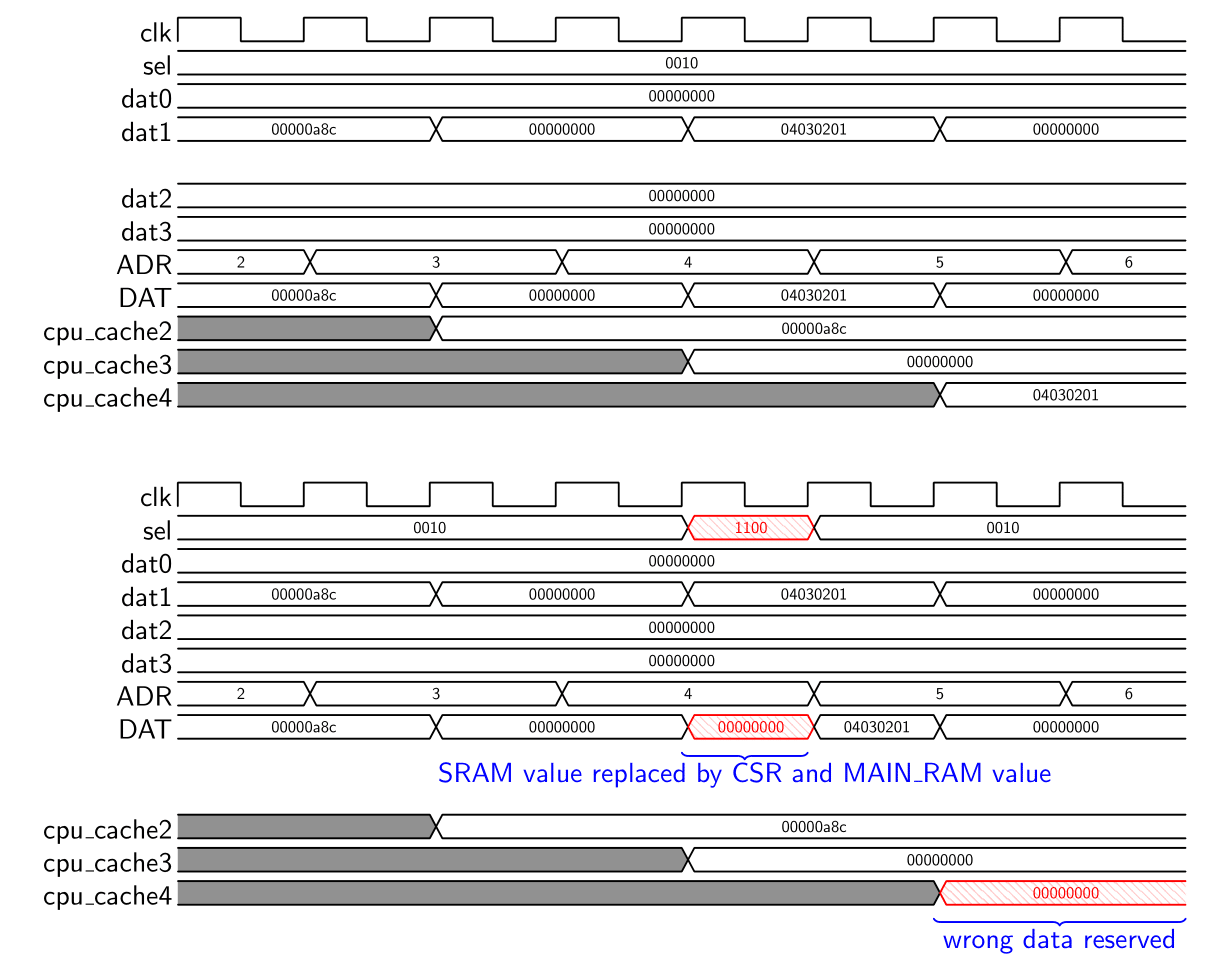
\includegraphics[width=\linewidth]{Chapitre4/figures/fault5.png}
  \caption{Impact of data multiread on selection signal, data signals and CPU cache with/without attack}
  \label{fault5}
\end{figure}

In general, attack on is \texttt{SEL} equivalent to multiple bit-resets/multiple bit-flips at RTL level and instruction replacement at instruction level. We can summarize two reasons for the success of the attack: the absence of a detector or corrector on the \texttt{ACK} and \texttt{SEL} signals; and the fact that the read bus does not use a multiplexer but a combinational logic gate. These disruptions demonstrate the critical impact of control signal vulnerabilities on the bus.

\begin{figure}[t!]
  \centering
  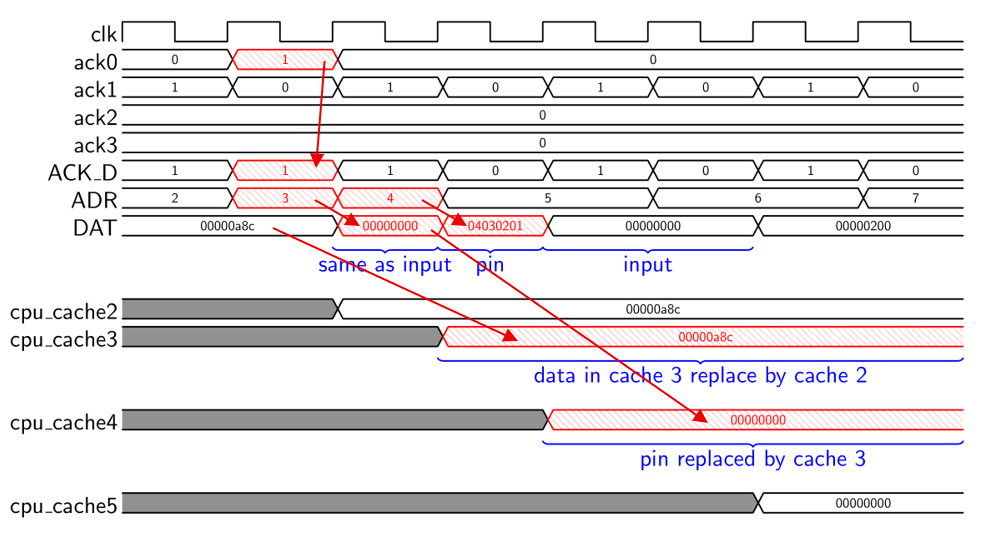
\includegraphics[width=\linewidth]{Chapitre4/figures/fault1.png}
  \caption{Impact of acknowledge signal on address, data signals and CPU cache without attack}
  \label{fault1}
\end{figure}

\begin{figure}[t!]
  \centering
  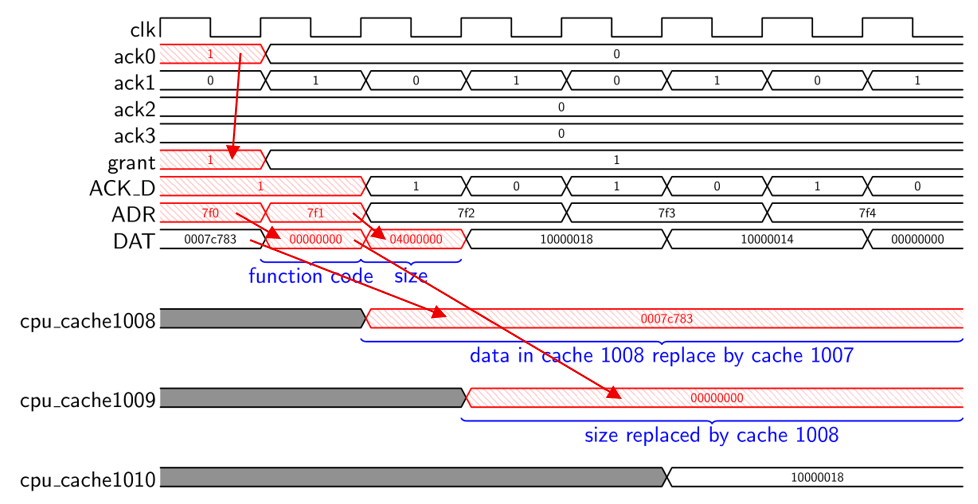
\includegraphics[width=\linewidth]{Chapitre4/figures/fault2.png}
  \caption{Impact of acknowledge signal on address, data signals and CPU cache with attack}
  \label{fault2}
\end{figure}

\section{Software countermeasures capacity against FIAs}

\subsection{Aim}
To effectively design countermeasures, we first analyze the sources and structures of vulnerability within the system. Our previous fault injection experiments reveal that attacks targeting the \texttt{ACK} and \texttt{SEL} signals can directly affect data flow integrity and control timing. These vulnerabilities arise from structural weaknesses: for instance, the absence of dedicated error detection or correction mechanisms on handshake and selection signals. Additionally, the \texttt{SEL} signal is controlled by a purely combinational multiplexer without any built-in verification logic. Such architectural choices leave the system particularly susceptible to fault injection that manipulates signal timing or selectively disables data paths, leading to corrupted reads and logical bypasses.

While implementing hardware-level countermeasures is possible, it often comes at a high resource cost, especially in lightweight embedded systems where logic and memory budget is constrained. In contrast, the existing \texttt{VerifyPin} benchmark already includes a software-level countermeasure designed to address software-based attacks, even though such attacks are outside the scope of this research. Nevertheless, these software countermeasures offer a valuable line of defense and can be extended to mitigate certain fault-induced vulnerabilities. Therefore, we choose to first implement a software-based countermeasure, as it provides a low-overhead solution compatible with the current system architecture and lays the foundation for evaluating integrated fault resilience.

\subsection{Countermeasure introduction}
The VerifyPin benchmark incorporate various countermeasures to enhance resilience against software attacks:

\begin{enumerate}
\item HB (Hardened Booleans): This technique encodes Boolean values using two constants with a high Hamming distance, making it more challenging to switch between values with a single fault injection. The primary objective is to protect against data-modifying faults.

\item FTL (Fixed-Time Loop): This countermeasure ensures that an algorithm's execution time remains constant regardless of the input data, thereby mitigating timing analysis attacks. By preventing variations in execution time, attackers are unable to infer sensitive information such as encryption keys. In the actual program, they implement this protection by verifying that the number of loops is correct.

\item INL (Inlined Functions): Function calls are replaced with their corresponding function code, reducing the attack surface. This countermeasure protects against instruction-skipping attacks on function calls by eliminating the instructions used to pass parameters during calls.

\item DPTC (PTC Decremented First): PTC refers to a counter used to regulate program loops or execution times. By decreasing the counter before entering critical code, the system prevents attackers from creating infinite loops or time exceptions through instruction skipping or unauthorized instruction insertion.

\item PTCBK (PTC Backup): This countermeasure safeguards against counter tampering or rollback attacks. By maintaining a backup of counter values, the system can revert to a trusted state if anomalies are detected. If the backup value differs from the current counter value, protective measures such as execution interruption can be triggered. In the actual program (V4), it copies the value of the counter to another variable, reduces the values of both and compares them to achieve this measure.

\item LC (Loop Counter): This mechanism monitors and limits the number of loop executions in a program to prevent infinite loops or excessive resource consumption. The system records the loop count during execution and triggers safety measures if the count exceeds predefined limits, thereby avoiding resource exhaustion or abnormal behavior.

\item DC (Double Call): To prevent tampering during critical function calls, the program executes two identical calls and compares their results. If the outcomes differ, the program identifies a potential attack or tampering attempt and may trigger protective responses.

\item DT (Double Test): This countermeasure ensures data integrity by performing two evaluations for key conditions. If the results differ, it indicates possible tampering, prompting the system to raise alarms or take protective measures.

\item SC (Step Counter): This technique monitors the number or sequence of critical program steps to prevent process control tampering. If the Step Counter deviates from the expected value, the system may abort execution or enter a protective mode to maintain operational security.
\end{enumerate}

As shown in Table~\ref{tab:benchmark cm}, A detailed explanation of each countermeasure is provided below.

\begin{table}
  \caption{Software countermeasures deployed in each benchmark version}
  \label{tab:benchmark cm}
  \begin{tabular}{cccccccccc}
    \hline
    & HB & FTL & INL & DPTC & PTCBK & LC & DC & DT & SC\\
    \hline
    \texttt{v0} & & & & & & & & &  \\
    \texttt{v1} & \checkmark & & & & & & & &  \\
    \texttt{v2} & \checkmark & \checkmark & & & & & & & \\
    \texttt{v3} & \checkmark & \checkmark & \checkmark & & & & & & \\
    \texttt{v4} & \checkmark & \checkmark & \checkmark & \checkmark & \checkmark & \checkmark & & &\\
    \texttt{v5} & \checkmark & \checkmark & & \checkmark & & & \checkmark & &  \\
    \texttt{v6} & \checkmark & \checkmark & \checkmark & \checkmark & & & & \checkmark &  \\
    \texttt{v7} & \checkmark & \checkmark & \checkmark & \checkmark & & & & \checkmark & \checkmark\\
    \hline
  \end{tabular}
\end{table}

In Figure\ref{V0}, we reuse the code.c file to show the countermeasure implement in other versions.
\begin{figure}
\begin{lstlisting}[caption={code.c of VerifyPin function in benchmark V0}, label={V0}, basicstyle=\ttfamily\footnotesize]
#include "interface.h"
#include "types.h"
#include "commons.h"

extern SBYTE g_ptc;
extern BOOL g_authenticated;
extern UBYTE g_userPin[PIN_SIZE];
extern UBYTE g_cardPin[PIN_SIZE];

#ifdef INLINE
__attribute__((always_inline)) inline BOOL byteArrayCompare(UBYTE* a1, UBYTE* a2, UBYTE size)
#else
BOOL byteArrayCompare(UBYTE* a1, UBYTE* a2, UBYTE size)
#endif
{
    int i;
    for(i = 0; i < size; i++) {
        if(a1[i] != a2[i]) {
            return 0;
        }
    }
    return 1;
}

BOOL verifyPIN() {
    g_authenticated = 0;

    if(g_ptc > 0) {
        if(byteArrayCompare(g_userPin, g_cardPin, PIN_SIZE) == 1) {
            g_ptc = 3;
            g_authenticated = 1; // Authentication();
            return 1;
        } else {
            g_ptc--;
            return 0;
        }
    }

    return 0;
}
\end{lstlisting}
\end{figure}

In Version 1 Figure\ref{V1}, the HB countermeasure is implemented at lines 19 and 22. We replace the original return values 0 and 1 with the Boolean constants false and true. This modification allows us to verify whether the variable comp is altered to any unexpected value outside the Boolean domain. By doing so, we can detect potential fault attacks that attempt to manipulate comp to bypass verification logic.

\begin{figure}
\begin{lstlisting}[caption={code.c of VerifyPin function in benchmark V1}, label={V1}, basicstyle=\ttfamily\footnotesize]
#include "interface.h"
#include "types.h"
#include "commons.h"

extern SBYTE g_ptc;
extern BOOL g_authenticated;
extern UBYTE g_userPin[PIN_SIZE];
extern UBYTE g_cardPin[PIN_SIZE];

#ifdef INLINE
 __attribute__((always_inline)) inline BOOL byteArrayCompare(UBYTE* a1, UBYTE* a2, UBYTE size)
#else
BOOL byteArrayCompare(UBYTE* a1, UBYTE* a2, UBYTE size)
#endif
{
    int i;
    for(i = 0; i < size; i++) {
        if(a1[i] != a2[i]) {
            return BOOL_FALSE;
        }
    }
    return BOOL_TRUE;
}

BOOL verifyPIN() {
    int comp;
    g_authenticated = BOOL_FALSE;

    if(g_ptc > 0) {
        comp = byteArrayCompare(g_userPin, g_cardPin, PIN_SIZE);
        if(comp == BOOL_TRUE) {
            g_ptc = 3;
            g_authenticated = BOOL_TRUE; // Authentication();
            return BOOL_TRUE;
        } else if(comp == BOOL_FALSE) {
          g_ptc--;
          return BOOL_FALSE;
        } else {
          countermeasure();
        }
    }
    return BOOL_FALSE;
}
\end{lstlisting}
\end{figure}

In Version 2 (Figure \ref{V2}), the HB countermeasure is implemented in the same way as in Version 1. In addition to this, FTL protection is introduced. Specifically, after the loop concludes, a check is performed at line 25 to verify whether the loop counter has reached the expected value. This serves to detect any premature termination of the loop that could be caused by a fault injection attack.

\begin{figure}
\begin{lstlisting}[caption={code.c of VerifyPin function in benchmark V2}, label={V2}, basicstyle=\ttfamily\footnotesize]
#include "interface.h"
#include "types.h"
#include "commons.h"

extern SBYTE g_ptc;
extern BOOL g_authenticated;
extern UBYTE g_userPin[PIN_SIZE];
extern UBYTE g_cardPin[PIN_SIZE];
extern UBYTE g_countermeasure;

#ifdef LAZART
  __attribute__((always_inline)) inline BOOL byteArrayCompare(UBYTE* a1, UBYTE* a2, UBYTE size)
#else
  BOOL byteArrayCompare(UBYTE* a1, UBYTE* a2, UBYTE size)
#endif
{
    int i;
    BOOL status = BOOL_FALSE;
    BOOL diff = BOOL_FALSE;
    for(i = 0; i < size; i++) {
        if(a1[i] != a2[i]) {
            diff = BOOL_TRUE;
        }
    }
    if(i != size) {
        countermeasure();
    }
    if (diff == BOOL_FALSE) {
        status = BOOL_TRUE;
    } else {
        status = BOOL_FALSE;
    }

    return status;
}

BOOL verifyPIN()
{
    g_authenticated = BOOL_FALSE;

    if(g_ptc > 0) {
        if(byteArrayCompare(g_userPin, g_cardPin, PIN_SIZE) == BOOL_TRUE) {
            g_ptc = 3;
            g_authenticated = BOOL_TRUE; // Authentication();
            return BOOL_TRUE;
        } else {

            g_ptc--;
            return BOOL_FALSE;
        }
    }
    return BOOL_FALSE;
}
\end{lstlisting}
\end{figure}

In Version 3 (Figure \ref{V3}), both the HB and FTL countermeasures are implemented identically to Version 2. In addition to these, INL protection is introduced. Specifically, at line 33, instead of invoking the byteArrayCompare function, the comparison logic is written directly within the same function. This modification is intended to eliminate potential vulnerabilities that may arise during function calls, such as control-flow manipulation or return address corruption due to fault injection.

\begin{figure}
\begin{lstlisting}[caption={code.c of VerifyPin function in benchmark V3}, label={V3}, basicstyle=\ttfamily\footnotesize]
#include "interface.h"
#include "types.h"
#include "commons.h"

extern SBYTE g_ptc;
extern BOOL g_authenticated;
extern UBYTE g_userPin[PIN_SIZE];
extern UBYTE g_cardPin[PIN_SIZE];

BOOL verifyPIN() {
    int i;
    BOOL status;
    BOOL diff;
    g_authenticated = BOOL_FALSE;

    if(g_ptc > 0) {
        status = BOOL_FALSE;
        diff = BOOL_FALSE;
        for(i = 0; i < PIN_SIZE; i++) {
            if(g_userPin[i] != g_cardPin[i]) {
                diff = BOOL_TRUE;
            }
        }
        if(i != PIN_SIZE) {
            countermeasure();
        }
        if (diff == BOOL_FALSE) {
            status = BOOL_TRUE;
        } else {
            status = BOOL_FALSE;
        }

        if(status == BOOL_TRUE) {
            g_ptc = 3;
            g_authenticated = BOOL_TRUE; // Authentication();
            return BOOL_TRUE;
        } else {
            g_ptc--;
            return BOOL_FALSE;
        }
    }
    return BOOL_FALSE;
}
\end{lstlisting}
\end{figure}

In Version 4 (Figure \ref{V4}), the HB, FTL, and INL countermeasures are implemented in the same manner as in Version 2. In addition to these, three new protections are introduced: DPTC, PTCBK, and LC. Specifically, at line 22, the variable g\_ptc is decremented to help restore the system to a consistent internal state, thereby mitigating potential inconsistencies caused by an attack. At line 15, the value of g\_ptc is copied into a temporary variable ptcCpy, which is later checked to detect any unauthorized modifications, preventing tampering with the control variable. Finally, at line 35, a stepCounter variable is used to track the number of loop iterations, helping to detect and prevent control-flow faults that might cause the loop to be skipped or prematurely terminated.

\begin{figure}
\begin{lstlisting}[caption={code.c of VerifyPin function in benchmark V4}, label={V4}, basicstyle=\ttfamily\footnotesize]
#include "interface.h"
#include "types.h"
#include "commons.h"

extern SBYTE g_ptc;
extern BOOL g_authenticated;
extern UBYTE g_userPin[PIN_SIZE];
extern UBYTE g_cardPin[PIN_SIZE];

BOOL verifyPIN() {
    int i;
    BOOL status;
    BOOL diff;
    int stepCounter;
    SBYTE ptcCpy = g_ptc;
    g_authenticated = BOOL_FALSE;

    if(g_ptc > 0) {
        if(ptcCpy != g_ptc) {
            countermeasure();
        }
        g_ptc--;
        if(g_ptc != ptcCpy-1) {
            countermeasure();
        }
        ptcCpy--;

        status = BOOL_FALSE;
        diff = BOOL_FALSE;
        stepCounter = 0;
        for(i = 0; i < PIN_SIZE; i++) {
            if(g_userPin[i] != g_cardPin[i]) {
                diff = BOOL_TRUE;
            }
            stepCounter++;
        }
        if(stepCounter != PIN_SIZE) {
            countermeasure();
        }
        if(i != PIN_SIZE) {
            countermeasure();
        }
        if (diff == BOOL_FALSE) {
            status = BOOL_TRUE;
        } else {
            status = BOOL_FALSE;
        }

        if(status == BOOL_TRUE) {
            if(ptcCpy != g_ptc) {
                countermeasure();
            }
            g_ptc = 3;
            g_authenticated = BOOL_TRUE; // Authentication();
            return BOOL_TRUE;
        }
    }

    return BOOL_FALSE;
}
\end{lstlisting}
\end{figure}

In Version 5 (Figure \ref{V5}), DC protection is introduced. Specifically, at line 42, the byteArrayCompare function is called twice consecutively to obtain two results. This redundancy helps to detect and prevent fault injection attacks targeting the function call itself.

\begin{figure}
\begin{lstlisting}[caption={code.c of VerifyPin function in benchmark V5}, label={V5}, basicstyle=\ttfamily\footnotesize]
#include "interface.h"
#include "types.h"
#include "commons.h"

extern SBYTE g_ptc;
extern BOOL g_authenticated;
extern UBYTE g_userPin[PIN_SIZE];
extern UBYTE g_cardPin[PIN_SIZE];

#ifdef INLINE
__attribute__((always_inline)) inline BOOL byteArrayCompare(UBYTE* a1, UBYTE* a2, UBYTE size)
#else
BOOL byteArrayCompare(UBYTE* a1, UBYTE* a2, UBYTE size)
#endif
{
    int i;
    BOOL status = BOOL_FALSE;
    BOOL diff = BOOL_FALSE;
    for(i = 0; i < size; i++) {
        if(a1[i] != a2[i]) {
            diff = BOOL_TRUE;
        }
    }
    if(i != size) {
        countermeasure();
    }
    if (diff == BOOL_FALSE) {
        status = BOOL_TRUE;
    } else {
        status = BOOL_FALSE;
    }
    return status;
}

BOOL verifyPIN() {
    g_authenticated = BOOL_FALSE;

    if(g_ptc > 0) {
        g_ptc--;

        if(byteArrayCompare(g_userPin, g_cardPin, PIN_SIZE) == BOOL_TRUE) {
            if(byteArrayCompare(g_cardPin, g_userPin, PIN_SIZE) == BOOL_TRUE) {
                g_ptc = 3;
                g_authenticated = BOOL_TRUE; // Authentication();
                return BOOL_TRUE;
            } else countermeasure();
        }
    }

    return BOOL_FALSE;
}
\end{lstlisting}
\end{figure}

In Version 6 (Figure \ref{V6}), DT protection is implemented. Specifically, at lines 30 and 40, the values diff and status are compared twice consecutively to detect and prevent fault injection attacks targeting the comparison operations.

\begin{figure}
\begin{lstlisting}[caption={code.c of VerifyPin function in benchmark V6}, label={V6}, basicstyle=\ttfamily\footnotesize]
#include "interface.h"
#include "types.h"
#include "commons.h"

extern SBYTE g_ptc;
extern BOOL g_authenticated;
extern UBYTE g_userPin[PIN_SIZE];
extern UBYTE g_cardPin[PIN_SIZE];

BOOL verifyPIN() {
    int i;
    BOOL status;
    BOOL diff;
    g_authenticated = BOOL_FALSE;

    if(g_ptc > 0) {
        g_ptc--;

        status = BOOL_FALSE;
        diff = BOOL_FALSE;
        for(i = 0; i < PIN_SIZE; i++) {
            if(g_userPin[i] != g_cardPin[i]) {
                diff = BOOL_TRUE;
            }
        }
        if(i != PIN_SIZE) {
            countermeasure();
        }
        if (diff == BOOL_FALSE) {
            if(BOOL_FALSE == diff) {
                status = BOOL_TRUE;
            } else {
                countermeasure();
            }
        } else {
            status = BOOL_FALSE;
        }

        if(status == BOOL_TRUE) {
            if(BOOL_TRUE == status) {
                g_ptc = 3;
                g_authenticated = BOOL_TRUE; // Authentication();
                return BOOL_TRUE;
            } else {
                countermeasure();
            }
        }
    }

    return BOOL_FALSE;
}
\end{lstlisting}
\end{figure}

In Version 7 (Figure \ref{V7}), SC protection is implemented. Specifically, a variable stepCounter is used to track the number of executed actions. After execution, the value of stepCounter is verified to ensure correctness. This mechanism effectively mitigates nearly all types of instruction skip attacks occurring at the line level.

\begin{figure}
\begin{lstlisting}[caption={code.c of VerifyPin function in benchmark V7}, label={V7}, basicstyle=\ttfamily\footnotesize]
#include "interface.h"
#include "types.h"
#include "commons.h"

extern SBYTE g_ptc;
extern BOOL g_authenticated;
extern UBYTE g_userPin[PIN_SIZE];
extern UBYTE g_cardPin[PIN_SIZE];

BOOL verifyPIN() {
    int stepCounter = 0;
    int i;
    BOOL status;
    BOOL diff;
    g_authenticated = BOOL_FALSE;

    if(g_ptc > 0) {
        stepCounter++;
        if(stepCounter != 1) {
            countermeasure();
        }
        g_ptc--;
        stepCounter++;
        if(stepCounter != 2) {
            countermeasure();
        }

        status = BOOL_FALSE;
        diff = BOOL_FALSE;

        stepCounter++;
        if(stepCounter != 3) {
            countermeasure();
        }

        for(i = 0; i < PIN_SIZE; i++) {
            if(g_userPin[i] != g_cardPin[i]) {
                diff = BOOL_TRUE;
            }
            stepCounter++;
            if(stepCounter != i+4) {
                countermeasure();
            }
        }
        stepCounter++;
        if(stepCounter != 4+PIN_SIZE) {
            countermeasure();
        }
        if(i != PIN_SIZE) {
            countermeasure();
        }
        if (diff == BOOL_FALSE) {
            if(BOOL_FALSE == diff) {
                status = BOOL_TRUE;
            } else {
                countermeasure();
            }
        } else {
            status = BOOL_FALSE;
        }
        stepCounter++;
        if(stepCounter != 5+PIN_SIZE) {
            countermeasure();
        }

        if(status == BOOL_TRUE) {
            stepCounter++;
            if(stepCounter != 6+PIN_SIZE) {
                countermeasure();
            }
            if(BOOL_TRUE == status) {
                stepCounter++;
                if(stepCounter != 7+PIN_SIZE) {
                    countermeasure();
                }
                g_ptc = 3;
                stepCounter++;
                if(stepCounter != 8+PIN_SIZE) {
                    countermeasure();
                }
                g_authenticated = BOOL_TRUE; // Authentication();
                return BOOL_TRUE;
            } else {
                countermeasure();
            }
        } else {
            countermeasure();
        }
    }

    return BOOL_FALSE;
}
\end{lstlisting}
\end{figure}

\subsection{Step}
To initialize the formal verification process, we compile multiple versions of the VerifyPin benchmark (from V1 to V7) into formal model files. Throughout this process, the system configuration remains consistent with the previous setup, particularly regarding the Wishbone bus integration. Based on these settings, we proceed to generate the corresponding SoC in the form of a Verilog project, ensuring functional consistency and compatibility across all versions.

For automated fault injection, we utilize the FISSA framework. The target registers for injection are kept unchanged, as no structural modifications have been made to the architecture itself. However, due to the increasing complexity and size of the application—especially after incorporating software countermeasures—we update the parameters \texttt{fenetre\_tir} and \texttt{cycle\_ref} within the configuration file \texttt{config\_wop.json}. Additionally, the comparison threshold against the variable \texttt{now} in the script \texttt{fault\_injection.py} is adjusted accordingly to align with the extended execution timeline of the newer program versions.

These configuration changes are summarized in Table~\ref{tab:variable configuration}, reflecting the necessary adjustments made to accommodate the increased program footprint and ensure consistent fault injection behavior across all benchmark iterations.

\begin{table}[]
  \caption{Difference in variable configuration in different version}
  \label{tab:variable configuration}
\begin{tabular}{rrrrr}
\multicolumn{1}{l}{version} & \multicolumn{1}{l}{from(fenetre\_tir)} & \multicolumn{1}{l}{to(fenetre\_tir)} & \multicolumn{1}{l}{threshold} & \multicolumn{1}{l}{cycle\_ref} \\
1 & 15870 & 18190 & 18264 & 2283 \\
2 & 15726 & 19390 & 19464 & 2433 \\
3 & 15694 & 18838 & 18912 & 2364 \\
4 & 15726 & 19918 & 19992 & 2499 \\
5 & 15678 & 19166 & 19240 & 2405 \\
6 & 15806 & 19014 & 19088 & 2386 \\
7 & 6062 & 14486 & 15504 & 1938
\end{tabular}
\end{table}

Because we add countermeasure, we change simulation results classification:
\begin{enumerate}
\item Crash, the simulation either exceeded the fixed execution time or triggered a crash signal, resulting in termination.
\item Detect, the fault was detected by the countermeasure, setting the variable \texttt{g\_countermeasure} to "1".
\item Success, the authentication bypassed successfully, with \texttt{g\_authenticated} set to "1".
\item Change, no successful authentication or detection occurred, but the memory state was altered by the fault.
\item Silence, no authentication success, detection, or memory state change was observed, indicating the fault had no visible impact.
\end{enumerate}

In parallel with the robustness testing of different benchmark versions, we employed the \texttt{Lizard} tool~\cite{Lizard} to analyze their code complexity and computational cost. The complexity metrics for each benchmark are presented in Table~\ref{tab:benchmark result}. \texttt{Lizard} provides a detailed analysis across various parameters, which are described as follows:
\begin{enumerate}
\item NLOC (Non-Commenting Lines of Code): This metric represents the total number of valid lines of code, excluding blank lines and comments. It serves as a direct indicator of code size and readability.

\item CCN (Cyclomatic Complexity Number): This metric measures the McCabe complexity of all functions, which reflects the number of independent logical paths within a program. Higher CCN values indicate greater logical complexity, making the code more challenging to maintain and test.

\item Token Count: This parameter represents the total number of lexical units, including operators, operands, and other functional elements. It provides insight into the syntactic complexity of the program.
\end{enumerate}

We install the \texttt{Lizard} analysis tool on a Linux-based system to evaluate code complexity metrics across different versions of the \texttt{VerifyPin} benchmark. For each version, \texttt{Lizard} is executed within the corresponding source directory. This process allows us to extract key software metrics such as function count, cyclomatic complexity, and lines of code, which are later used for comparative analysis. The extracted elements are consistent with those previously defined.

\subsection{Result}

The experimental results validate the initial hypothesis that the vulnerabilities are primarily concentrated on the \texttt{ACK}, \texttt{grant} and \texttt{SEL} signals. A detailed evaluation of the condition numbers is presented in Table~\ref{tab:benchmark result}. Among the eight benchmark versions, V7 exhibited the lowest fault injection success rate, whereas V4 achieved the highest fault detection capability. Further examination revealed a notable relationship between the complexity of the countermeasures—measured by code length, cyclomatic complexity (CCN), and token count—and the total number of required simulation cycles. As the countermeasures became more elaborate, program execution time increased, inadvertently expanding the fault injection surface.

Interestingly, certain countermeasures that lacked alignment with the specific characteristics of the fault model—failing to effectively intercept or neutralize relevant fault paths—produced higher success rates than even the baseline versions without protection, such as V1 and V5. This counterintuitive outcome implies that while the fundamental fault model remained consistent, none of the implemented countermeasures succeeded in fully neutralizing the fault impact. These findings highlight the necessity for a more granular analysis of each countermeasure’s logic and deployment in order to uncover the underlying reasons behind this anomalous behavior.

\begin{table*}
  \centering
  \caption{Fault injection results and code complexity metrics for each benchmark version}
  \label{tab:benchmark result}
\begin{tabular}{ccccccccccc}
\hline
& crash & detect & success & change & silence & success rate & sum & NLOC & CCN & token \\
\hline
V0 & 43 & 0 & 24 & 69 & 2438 & 0.93\% & 2574 & 32 & 6 & 107 \\
V1 & 68 & 19 & 37 & 103 & 2963 & 1.16\% & 3190 & 36 & 7 & 127 \\
V2 & 88 & 16 & 50 & 124 & 4760 & 0.99\% & 5038 & 44 & 8 & 149 \\
V3 & 81 & 23 & 15 & 109 & 4095 & 0.35\% & 4323 & 32 & 7 & 129 \\
V4 & 94 & 125 & 17 & 88 & 5440 & 0.29\% & 5764 & 47 & 11 & 191 \\
V5 & 92 & 27 & 39 & 114 & 4524 & 0.81\% & 4796 & 42 & 9 & 163 \\
V6 & 78 & 22 & 10 & 97 & 4204 & 0.23\%  & 4411 & 38 & 9 & 153 \\
V7 & 110 & 200 & 5 & 99 & 9673 & 0.05\% & 10087 & 77 & 18 & 312\\       
\hline                          
\end{tabular}
\end{table*}

\begin{table*}
  \centering
  \caption{Skipped instructions caused by attacks in V0, V1, V4, and V5 benchmarks}
  \label{tab:fault analysis}
\resizebox{\textwidth}{!}{%
\begin{tabular}{llllcc}
    \hline
& skipped instruction & code correct & code corrupt & code line & new fault \\
    \hline
& li a5, 1 & if(function == 1) & if(function == \textcolor{red}{0}) & 10 &\\
& bne a4, a5, loc\_1FC & if(function == 1) & jump to \textcolor{red}{ g\_authenticated = 1} & 10 &\\
& lbu a5, 20h+size(sp) & if (i \textless size) & if (i \textless \textcolor{red}{ i}) & 2 &\\
\multirow{-4}{*}{V0} & li a5, 0 & return 0 & return \textcolor{red}{ 1} & 3 &\\
\hline

& li a5, 1 & if(comp == 1) & if(comp == \textcolor{red}{ 0}) & 11 &\\
& bne a4, a5, loc\_200 & if(comp == 1) & jump to \textcolor{red}{ g\_authenticated = 1} & 11 &\\
& mv a5, a2 & store size value as 4 & store size value as \textcolor{red}{0} & 1 & \checkmark\\
& sb a5, 20h+size(sp) & store size value as 4 & store size value as \textcolor{red}{ random} & 1 & \checkmark\\
& li a5, 0 & return 0 & return \textcolor{red}{ 1} & 3 &\\
& j loc\_18C & jump to return 0 & jump to \color[HTML]{FF0000} {next loop} & 3 & \checkmark\\
& lbu a5, 20h+size(sp) & if (i \textless size) & if (i \textless \textcolor{red}{ i}) & 2 &\\
\multirow{-8}{*}{V1} & sw a5, 1Ch+comp(sp) & comp = 0 & comp =\textcolor{red}{ random} & 10 & \checkmark\\
\hline

& sb a5, 1Ch+diff(sp) & diff = 1 & diff = \textcolor{red}{ random} & 12 & \\
& bnez a5, loc\_258 & if (diff == 0) & jump to \textcolor{red}{ status = 1} & 16 &\\      
\multirow{-3}{*}{V4} & bne a4, a5, loc\_29C & if (status = 1) & jump to \textcolor{red}{ g\_authenticated = 1} & 18 &\\
\hline

& mv a5, a2 & store size value as 4 & store size value as \textcolor{red}{ random} & 1 & \checkmark\\
& sb a5, 2Ch+size(sp) & store size value as 4 & store size value as \textcolor{red}{ 0} & 1 & \checkmark\\
& lbu a5, 2Ch+size(sp) & if (i \textless size) & if (i \textless \textcolor{red}{ i}) & 4 & \checkmark\\
& sb a5, 2Ch+diff(sp) & diff = 1 & diff = \textcolor{red}{ random} & 5 &\\
& bnez a5, loc\_1B8 & if (diff == 0) &  jump to \textcolor{red}{ status = 1} & 8 &\\
& sb zero, 2Ch+status(sp) & status = 0 & status = \textcolor{red}{ random} & 9 & \checkmark\\
\multirow{-7}{*}{V5} & lbu a5, 2Ch+status(sp) & status = 0 & status = \textcolor{red}{ 1} & 9 & \checkmark\\ 
\hline
\end{tabular}
}
\end{table*}

Across all benchmark versions, successful fault injections were observed to impact both data signals originating from SRAM and instruction signals sourced from ROM. As previously discussed, data-related vulnerabilities are primarily induced by faults on the \texttt{ACK} and \texttt{SEL} signals. However, given that the frequency of successful data attacks remains largely consistent across all versions, these do not appear to be the dominant contributors to the observed differences in attack success rates.

In comparison, instruction-level vulnerabilities exert a more substantial influence. These faults are predominantly associated with "skip-repeat" behavior triggered by instruction-level disruptions—most notably, those induced by \texttt{ACK} faults. Since many repeated instructions (e.g., arithmetic, logical, and comparison operations) are inherently idempotent, their unintended repetition often leaves program behavior unchanged. The more critical consequence arises from instruction skipping, which more significantly compromises program integrity and thus increases the likelihood of attack success.

A comprehensive overview of all identified fault vulnerabilities is provided in Table~\ref{tab:fault analysis}. This includes the relevant assembly sequences used in fault payloads, associated code fragments, the specific code locations where the faults manifest, and an indication of whether each vulnerability was previously known or newly identified in this work.

From V0 (Listing~\ref{V0}) to V1 (Listing~\ref{V1}), a hardened Boolean countermeasure was introduced to protect the result of the function that compares the user PIN and the card PIN from being easily manipulated (V1 lines 19). This countermeasure mitigates attacks that exploit instruction skipping on the else branch. However, attacks that skip the comparison condition—\texttt{if(function == 1)} (V0 line 29) and \texttt{if(comp == 1)} (V1 line 31)—remain undetected. Additionally, faults such as skipping instructions responsible for reading constant values (line 17 in V0 and in V1), the variable \texttt{size} (line 13 in V0 and in V1), or the return value (line 19 in V0 and V1) are not protected and remain exploitable. Furthermore, the increased instruction count in V1 introduces new vulnerable locations (marked as "new fault" in Table \ref{tab:fault analysis}), creating additional fault injection opportunities. As a result, the attack success rate in V1 unexpectedly increases rather than decreases.

A similar trend is observed when comparing V4 in Listing~\ref{V4} to V5 in Listing~\ref{V5}. In V5, three countermeasures — backup counter value, inlined calls and loop counter (V4 lines 22, 31, 35)  — were removed, while a new countermeasure, double call, was introduced in line 33. The removal of the loop counter eliminated protection on the loop counter variable, which allows fault injection to manipulate the statement \texttt{if (i < size)}(V5 line 19). It controls loop iterations, potentially forcing premature loop termination. The exclusion of inlined calls increased the instruction count for reading the variables \texttt{size} and \texttt{status}, exposing these operations to instruction-skipping attacks that assign unintended random values. Although the backup counter value on variable \texttt{g\_ptc} was removed, this did not affect the attack success rate since no attacks were observed targeting \texttt{g\_ptc}. Notably, while V4 was vulnerable to attacks on the code \texttt{if(status == true)} in line 49, the introduction of the double call countermeasure in V5 successfully mitigated similar attacks on the corresponding instruction. However, the code \texttt{diff = true} (V4 line 33, V5 line 21) and \texttt{if(diff == false)} (V4 line 43, V5 line 27) remained unprotected across both versions, leaving them vulnerable to fault injection attacks. Overall, the changes in countermeasures introduced more vulnerabilities than they mitigated, resulting in a higher attack success rate in V5.

A comparative evaluation of the countermeasures applied against hardware-induced faults targeting protected instructions is presented in Table~\ref{tab:cm evaluate}. Our experimental findings indicate that the implemented protections—\texttt{INL}, \texttt{LC}, \texttt{DC}, \texttt{DT}, and \texttt{SC}—when applied to critical operations such as comparison checks and loop control, are generally effective in addressing instruction-level vulnerabilities characterized by the skip-repeat fault model.

Nonetheless, it is crucial to recognize that the observed effectiveness is influenced by the nature of the test programs and the specific deployment of each countermeasure. A method that appeared less effective in our benchmarks might yield better results if repositioned or more tightly integrated within different code structures. Moreover, since these software-based defenses function at the instruction granularity, while hardware faults—even when modeled as single bit-flips—can propagate across multiple instructions, the protective scope of these mechanisms is inherently limited. This structural mismatch between fault impact and protection granularity underpins the incomplete mitigation observed in our evaluation.

\begin{table}
  \caption{Evaluation of software countermeasures against hardware fault attacks}
  \label{tab:cm evaluate}
\begin{tabular}{ccccccccc}
    \hline
HB & FTL & INL & DPTC & PTCBK & LC & DC & DT & SC \\
    \hline
x  & x   &  \checkmark   & x    & x     & \checkmark   &  \checkmark  &  \checkmark  &  \checkmark \\
    \hline
\end{tabular}
\end{table}

\section{Proposed hardware countermeasures based on multiplexer and redundant mechanisms}

\subsection{Aim}

In our experiments, we evaluated the effectiveness of various software countermeasures under fault injection. Surprisingly, even the most robust implementation—Version 7, which includes enhanced step verification and redundancy—failed to fully defend against the simplest fault model: a single bit-flip. This highlights a critical limitation of software-only approaches. While software countermeasures can raise the difficulty of successful attacks, they are inherently constrained by their reliance on the same vulnerable execution platform they aim to protect.

Given these limitations, hardware-based countermeasures must be seriously considered as a complementary or even primary defense strategy. In the following section, we will first review several commonly adopted hardware protection techniques, such as redundancy, error detection and correction, and bus integrity monitoring. After that, we will analyze the system's resilience when only hardware-level protections are deployed, offering a baseline for evaluating the combined effectiveness of hardware and software countermeasures.

\subsection{Countermeasure introduction}
In Section 4.1, we identified that the primary vulnerabilities stem from the lack of detection mechanisms for the \texttt{ACK} and \texttt{SEL} signals, as well as the combinational multiplexer in the read bus. To address these vulnerabilities, we modified the architecture to mitigate multiple read attacks (as shown in Figure~\ref{change archi}). Previously, the structure involved 4-bit \texttt{SEL} signals directly accessing registers, which were then connected to various memories through an OR gate. In the updated design, the 4-bit signal first passes through a 4-to-2 encoder  before being fed into the register, which serves as the selector signal for the four memories in the multiplexer (Figure \ref{change archi}). Following this architectural change, we applied various hardware countermeasures such as parity and duplication to the \texttt{ACK} and \texttt{SEL} registers. 

\begin{figure}[t!]
  \centering
  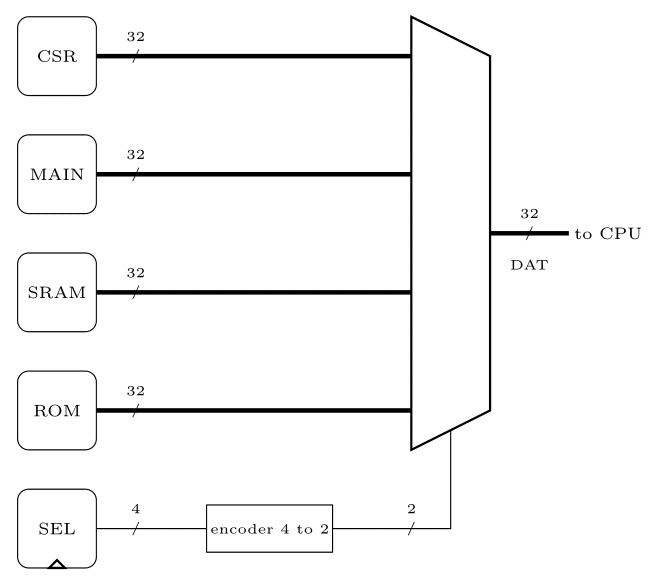
\includegraphics[width=0.9\linewidth]{Chapitre4/figures/change arch.png}
  \caption{Optimized connection between selection register and memory using multiplexers}
  \label{change archi}
\end{figure}

We employed six different countermeasures for the \texttt{ACK} and \texttt{SEL} registers:
\begin{enumerate}
\item Simple Parity: Detects faults using a 1-bit parity code.
\item Duplication: Creates a duplicate of the registers and compares it with the unprotected version. In Figure~\ref{cm archi}, the \texttt{SEL} signal is duplicated after the encoder, and the duplicated 2-bit signal is stored in the \texttt{cm} register. The signals in both registers are then compared to verify the integrity of the \texttt{SEL} signal and ensure it has not been tampered with. The comparison result is subsequently transmitted to the CPU.
\item Complementary Duplication: Duplicates the inverse of the registers and compares it with the unprotected version.
\item Hamming Code: Corrects the output signal of a register using a 3-bit checksum.
\item SECDED Code: Corrects or detects errors using a 4-bit checksum.
\item Triplication: Duplicates a register twice, correcting the signal if two registers have matching outputs and detecting errors if all three differ.
\end{enumerate}

\begin{figure}[t!]
  \centering
  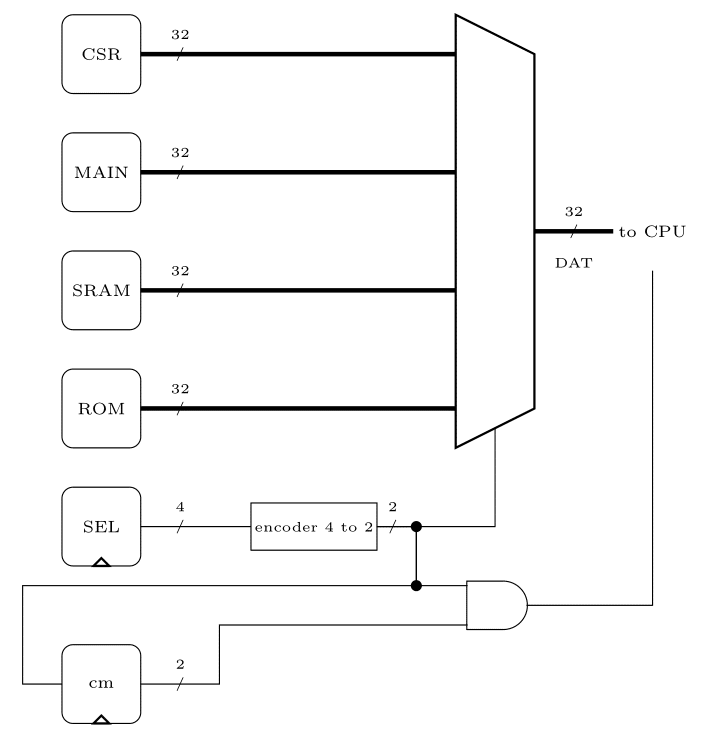
\includegraphics[width=0.9\linewidth]{Chapitre4/figures/cm.png}
  \caption{Structure of selection register and memory after deploying duplication countermeasure}
  \label{cm archi}
\end{figure}

\subsection{Step}
In our Verilog-based implementation, each hardware countermeasure was individually integrated into the \texttt{ACK} and \texttt{SEL} registers, resulting in six distinct project variants. Unlike software defenses, hardware protections function in real time, ensuring that simulation-time variables remain consistent across all configurations. However, introducing additional protection registers inevitably expands the attack surface, as these new elements may also become potential fault targets. To reflect these changes, we modified the register list in the YAML configuration file. We then employed FISSA to regenerate the corresponding TCL scripts and conducted fault injection campaigns using the Quastrasim simulation framework.

We performed a comprehensive analysis of the fault injection outcomes, focusing on several key metrics: the number of distinct fault conditions, attack success rate, detection rate, and correction rate. The experiment was conducted over a period of approximately one week, during which a total of 1,205,604 simulations were executed. Based on this dataset, we systematically compared the performance of different hardware countermeasures across multiple dimensions, as summarized below.

To further evaluate the cost of each countermeasure, we used Vivado to analyze resource utilization. Since resource overhead cannot be directly attributed to individual countermeasures, we synthesized and implemented full SoC designs containing each protection scheme, then compared the resulting differences in overall resource usage.

The experiments were carried out using Vivado version 2024.2 to ensure up-to-date toolchain support and synthesis accuracy. The SoC structure was specified as the top-level module. To obtain precise resource consumption metrics, we used post-implementation resource statistics rather than synthesis-only results. Based on the analysis, we identified and compared key resource categories including LUTs, flip-flops, and timing metrics such as Worst Negative Slack (WNS).

\begin{enumerate}
\item LUT (Look-Up Table): This represents the number of logic elements used to implement combinational logic. LUTs are the fundamental building blocks of FPGA logic, and their count reflects the complexity of the digital logic in the design.
\item Flip-Flop (FF): This indicates the number of sequential storage elements used in the design. Flip-flops store state information and are typically used for registers, control logic, and pipelines. The flip-flop count reflects the degree of sequential logic and pipelining.
\item WNS (Worst Negative Slack): This is a timing metric that shows the most critical timing violation, if any. A negative WNS means the design fails to meet timing requirements for at least one path. A positive or zero WNS indicates that the timing constraints are satisfied. Minimizing or eliminating WNS is essential to ensure reliable operation at the target clock frequency.
\end{enumerate}

Next, we need to calculate the maximum frequency for each structure. We adjust the clock cycle specified in the constraint file in Vivado, then run the implementation to make the WNS parameter closer to zero. The clock cycle obtained in this way is the minimum cycle in the ideal state, which gives us the maximum frequency.
\subsection{Result}

We derive the theoretical upper limit of possible bit-flip faults under the Manipulate Two Registers model, specifically when hardware-level countermeasures such as duplication, triplication, or SECDED are applied. In the most adversarial case, the attacker simultaneously compromises the \texttt{ACK} register (4 bits) and its corresponding redundancy register (4 bits), leading to a total of 8 potential bit-flips. Realistically, inducing such a level of disruption would require the attacker to align two independent fault injection pulses—such as laser beams or electromagnetic bursts—with high spatial and temporal accuracy, targeting both registers in perfect synchrony. As previously documented in the literature, achieving such dual-register precision is highly nontrivial, reinforcing the practical soundness of our threat model.

To evaluate the standalone performance of hardware-based countermeasures, we selected the V0 benchmark as the testing baseline, as it lacks any integrated software protection. The classification criteria for fault outcomes were maintained consistent with prior analysis. Detailed outcomes under varying fault conditions are shown in Table~\ref{tab:v0 under attack result}.

The table reveals significant distinctions in protective performance among the countermeasures. In general, duplication and complementary duplication yield lower attack success rates alongside higher detection probabilities. The Hamming code (SECDED) offers robust correction capability, particularly effective against dual-bit faults and distributed manipulations across two registers. Conversely, triplication is more effective when addressing single-bit errors and multi-bit corruption localized within a single register.

Certain countermeasures are particularly effective against specific attack types:
\begin{enumerate}
\item All countermeasures successfully defend against single bit-flip.
\item Duplication, complementary duplication, and triplication are effective against multi-bit manipulation within a single register.
\item SECDED can defend against two bit-flips.
\item No method can fully prevent multi-bit manipulation across two registers, but triplication performs better.
\end{enumerate}
However, some countermeasures remain vulnerable to specific attacks:
\begin{enumerate}
\item Simple Parity: Highly sensitive to two bit-flips, as simultaneous faults in both the parity and signal lines can compromise its effectiveness.
\item Hamming code and SECDED: Vulnerable to attacks that manipulate two registers, as large numbers of bit alterations can cause false corrections or mask faults in both the signal and the countermeasure.
\item Duplication, complementary duplication, and triplication: Susceptible to two bit-flips since injecting faults into two bits can mirror errors in the complement or duplicate registers, bypassing detection.
\end{enumerate}

\begin{table}
  \caption{Success, detection, and correction rates of hardware countermeasures in V0 benchmark under different fault models}
  \label{tab:v0 under attack result}
{%\footnotesize
\scriptsize
\begin{tabular}{llccl}
\hline
 &  & success rate & detect. rate & correct rate \\
\multirow{-2}{*}{countermeasure} & \multirow{-2}{*}{fault model} & (in \%) &(in \%) & (in \%)\\
\hline
 & bit-flip & 0.93 & &  \\
 & manipulate reg & 0.38 & & \\
 & 2 bit-flips & 1.39 & & \\
\multirow{-4}{*}{Unprotected} & manipulate 2 regs  & 0.71  &  & \\
\hline
 & bit-flip & 0 & 69.85 & \\
 & manipulate reg & 0.02 & 34.93 & \\
 & 2 bit-flips & 0.57 & 64.96 & \\
\multirow{-4}{*}{Simple parity} & manipulate 2 regs & 0.16 & 50.70 & \\
\hline
 & bit-flip & 0 & 77.89 & \\
 & manipulate reg & 0 & 45.11 & \\
 & 2 bit-flips & 0.10 & 86.87 & \\
\multirow{-4}{*}{Duplication} & manipulate 2 regs & 0.03 & 66.78 & \\
\hline
 & bit-flip & 0 & 77.89 & \\
Complimentary & manipulate reg & 0 & 45.11 & \\
duplication & 2 bit-flips & 0.10 & 86.87 & \\
 & manipulate 2 regs & 0.03 & 66.78 & \\
\hline
 & bit-flip & 0 & & 80 \\
 & manipulate reg & 0.31 & & 59.18 \\
 & 2 bit-flips & 0.62 & & 93.28 \\
\multirow{-4}{*}{Hamming code} & manipulate 2 regs & 0.64 & & 77.99 \\
\hline
 & bit-flip & 0 & 0 & 85.71 \\
 & manipulate reg & 0 & 0 & 81.82 \\
 & 2 bit-flips & 0.14 & 20 & 77.40 \\
\multirow{-4}{*}{Triplication} & manipulate 2 regs & 0.09 & 36.73 & 59.24 \\
\hline
 & bit-flip & 0 & 11.76 & 70.59 \\
 & manipulate reg & 0.21 & 34 & 38.56 \\
 & 2 bit-flips & 0 & 45.56 & 52.06 \\
\multirow{-4}{*}{Secded code} & manipulate 2 regs & 0.27 & 51.94 & 36.20 \\
\hline
\end{tabular}
}
\end{table}

The synthesis result is in Table~\ref{tab:countermeasures synthesis}. First, we observe that various countermeasures increase LUT usage by up to 0.7\% and reduce frequency by up to 0.97\% compared to the unprotected version. Considering the difference introduced by the synthesizer's auto-optimization, the countermeasure brings almost no additional hardware resource loss.

\begin{table}
    \centering
  \caption{Hardware resource overhead of each hardware countermeasure (LUT, flip-flop, frequency)}
  \label{tab:countermeasures synthesis}
\begin{tabular}{cccc}
\hline
countermeasure & LUT & flip-flop & frequency (MHz) \\
\hline
Unprotected & 2198 & 1793 & 70.13 \\
Simple parity & 2214 & 1791 & 70.27 \\
Duplication & 2201 & 1791 & 70.18 \\
Complimentary & 2199 & 1791 & 70.37 \\
Hamming code & 2199 & 1794 & 70.32 \\
Triplication & 2199 & 1791 & 70.27 \\
Secded code & 2193 & 1789 & 69.44 \\
\hline
\end{tabular}
\end{table}

\section{Comparison between hardware/software countermeasures}

\subsection{Aim}
Software countermeasures, while lightweight and resource-efficient, often provide only limited protection against fault attacks. They do not introduce additional hardware overhead, making them attractive for constrained environments, but their effectiveness diminishes when facing low-level or persistent fault models. In contrast, hardware countermeasures offer significantly stronger fault resilience by directly modifying the circuit structure or control flow. However, they come at the cost of increased resource consumption and still may not fully eliminate all attack vectors—especially under sophisticated or high-precision injection scenarios.

Given the limitations of each approach when used independently, we explore the possibility of combining software and hardware countermeasures to achieve a more balanced trade-off between protection capability and resource usage. Specifically, we investigate all possible combinations between the seven software countermeasure versions (V1 through V7) and the six hardware countermeasure implementations. Our goal is to determine whether any hybrid configuration can provide improved fault tolerance compared to standalone defenses, reduce the overall resource footprint compared to hardware-only implementations, or ideally, achieve both simultaneously.

\subsection{Step}
To explore the potential benefits of combining software and hardware countermeasures, we constructed a complete evaluation matrix by pairing seven different initialization files—each embedding a unique version of the software countermeasure—with seven Verilog-based SoC implementations, each integrating a distinct hardware countermeasure. The initialization files contain program code pre-instrumented with the corresponding software protections, while the Verilog projects incorporate hardware-level defenses into the SoC architecture, particularly around critical registers such as \texttt{ACK} and \texttt{SEL}.

For each of the 49 combined configurations, we utilized FISSA to generate the appropriate TCL scripts based on the matched software and hardware setup. Fault injection experiments were carried out using the Quastrasim simulation framework over the span of one month, resulting in over 20 million simulation runs in total.

The results were analyzed based on the number and type of fault conditions observed for each configuration. Key evaluation metrics include the attack success rate, detection rate, and correction rate across varying fault models. In parallel, we used Vivado to assess the hardware resource implications of each combination. The post-implementation reports provided detailed data on LUT usage, flip-flop count, and maximum achievable clock frequency, allowing for a comprehensive comparison of protection effectiveness versus hardware cost.

\subsection{Analysis}
Figure~\ref{hw cmp} displays the attack success rates observed under hardware-only countermeasures, while Figure~\ref{sw cmp} shows the corresponding results for software-only defenses. To facilitate a direct comparison between the two approaches, both bar charts are plotted using a unified vertical axis, with the scale limited to a maximum of 0.02.

When evaluating hardware and software countermeasures separately, it is evident that hardware-based protections consistently achieve lower attack success rates—often reaching zero in specific fault models. By contrast, none of the software countermeasures, including the most advanced version (V7), are able to fully eliminate any vulnerability model.

\begin{figure}[t!]
  \centering
  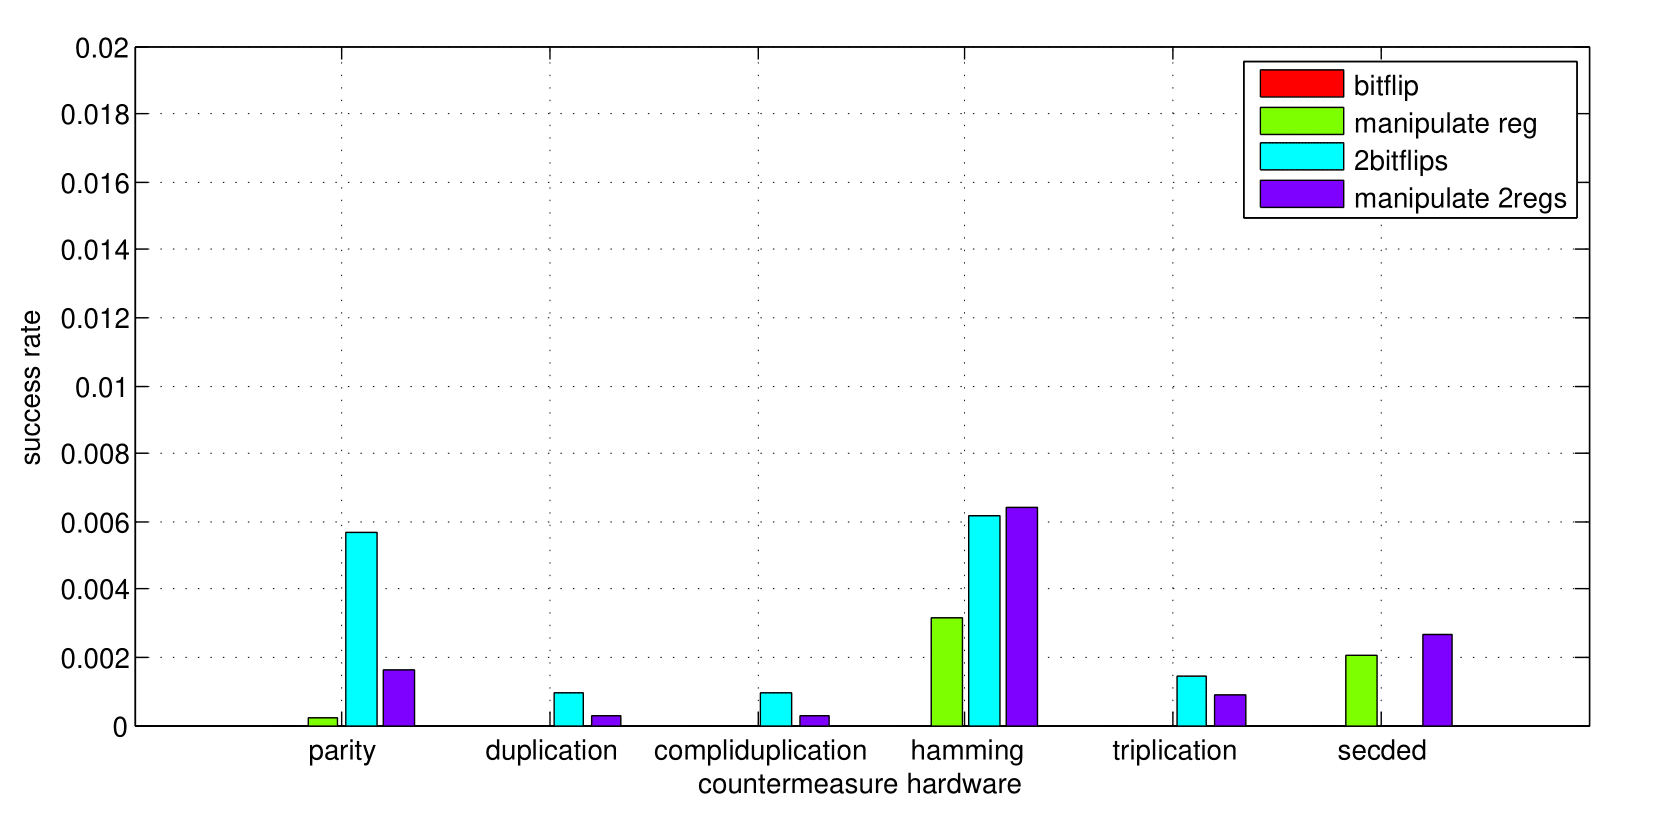
\includegraphics[width=0.99\linewidth]{Chapitre4/figures/hw rate.png}
  \caption{Success rates under four fault models for benchmark v0 with different hardware countermeasures}
  \label{hw cmp}
\end{figure}

\begin{figure}[t!]
  \centering
  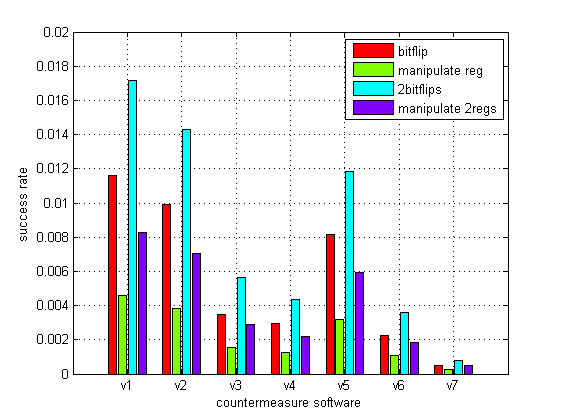
\includegraphics[width=0.99\linewidth]{Chapitre4/figures/sw rate.png}
  \caption{Success rates under four fault models for seven benchmark versions with software countermeasures}
  \label{sw cmp}
\end{figure}

Hardware-based countermeasures are capable of detecting or correcting faults almost instantaneously, with only minimal latency introduced by logic gate propagation delays. In contrast, software-based protections typically require more than 100 clock cycles to complete fault detection. However, considering that the overall program execution spans several thousand cycles, this additional latency is proportionally insignificant.

In terms of resource utilization, hardware countermeasures introduce limited overhead, primarily in the form of extra registers or combinational logic. On the other hand, software countermeasures result in only negligible memory overhead when compared to the total memory footprint of a real-world application. Based on these observations, we conclude that both hardware and software protections incur insignificant overheads—both in terms of execution time and resource consumption—within the scope of our experimental setup.

\begin{table*}
  \centering
  \caption{Success rates of manipulate register attacks on benchmarks with hardware countermeasures}
  \label{tab:manipulate}
\begin{tabular}{lllllllll}
\hline        
& V0 & V1 & V2 & V3 & V4 & V5 & V6 & V7 \\
\hline   
Unprotected                  & 0.385\%                                      & 0.460\%                                       & 0.386\%                                      & 0.153\%                                      & 0.127\%                                      & 0.321\%                                       & 0.108\%                                      & 0.029\%                                       \\
\hline
Simple parity             & 0.019\%                                      & 0.016\%                                       & 0.010\%                                      & 0.012\%                                      & 0.009\%                                      & 0.010\%                                       & 0.011\%                                      & 0.005\%                                        \\
\hline
Duplication               & 0                                              & 0                                              & 0                                              & 0                                              & 0                                              & 0                                              & 0                                              & 0                                              \\
\hline
Complimentary & 0                                              & 0                                              & 0                                              & 0                                              & 0                                              & 0                                              & 0                                              & 0                                              \\
\hline
Hamming code              & 0.314\%                                      & 0.385\%                                       & 0.328\%                                      & 0.120\%                                      & 0.101\%                                      & 0.270\%                                       & 0.081\%                                      & 0.019\%                                              \\
\hline
Triplication              & 0                                              & 0                                              & 0                                              & 0                                              & 0                                              & 0                                              & 0                                              & 0                                              \\
\hline
Secded code               & 0.205\%                                      & 0.255\%                                       & 0.218\%                                      & 0.076\%                                      & 0.065\%                                      & 0.179\%                                       & 0.050\%                                      & 0.037\% \\
\hline
\end{tabular}
\end{table*}

\begin{table*}
  \centering
  \caption{Success rates of 2 bit-flips attacks on benchmarks with hardware countermeasures}
  \label{tab:bitflips}
\begin{tabular}{lrrrrrrrr}
\hline
& V0 & V1 & V2 & V3 & V4 & V5 & V6 & V7 \\
                          \hline
Unprotected                  & 1.391\%                                      & 1.718\%                                       & 1.429\%                                      & 0.564\%                                      & 0.437\%                                       & 1.184\%                                       & 0.358\%                                       & 0.077\%                                       \\
\hline
Simple parity             & 0.567\%                                      & 0.746\%                                       & 0.595\%                                      & 0.254\%                                      & 0.187\%                                      & 0.492\%                                       & 0.159\%                                      & 0.030\%                                       \\
\hline
Duplication               & 0.098\%                                      & 0.122\%                                       & 0.104\%                                      & 0.036\%                                      & 0.031\%                                       & 0.085\%                                       & 0.024\%                                      & 0.005\%                                       \\
\hline
Complimentary & 0.098\%                                      & 0.122\%                                       & 0.104\%                                      & 0.036\%                                      & 0.031\%                                       & 0.085\%                                       & 0.024\%                                      & 0.005\%                                       \\
\hline
Hamming code              & 0.619\%                                      & 0.814\%                                       & 0.647\%                                       & 0.281\%                                      & 0.205\%                                      & 0.535\%                                       & 0.176\%                                      & 0.034\%                                       \\
\hline
Triplication              & 0.147\%                                      & 0.182\%                                       & 0.156\%                                      & 0.055\%                                      & 0.046\%                                      & 0.128\%                                       & 0.036\%                                      & 0.008\%                                       \\
\hline
Secded code               & 0                                              & 0                                              & 0                                              & 0                                              & 0                                              & 0                                              & 0                                              & 0  \\         
\hline
\end{tabular}
\end{table*}

\begin{table*}
  \centering
  \caption{Success rates of manipulate two registers attacks on benchmarks with hardware countermeasures}
  \label{tab:manipulates}
\begin{tabular}{lrrrrrrrr}
\hline
& V0 & V1 & V2 & V3 & V4 & V5 & V6 & V7\\
                          \hline
Unprotected                  & 0.606\%                                       & 0.830\%                                       & 0.703\%                                      & 0.287\%                                      & 0.218\%                                       & 0.591\%                                       & 0.185\%                                       & 0.047\%                                       \\
\hline
Simple parity             & 0.131\%                                      & 0.206\%                                      & 0.162\%                                      & 0.077\%                                      & 0.057\%                                      & 0.136\%                                       & 0.052\%                                      & 0.013\%                                       \\
\hline
Duplication               & 0.021\%                                      & 0.032\%                                       & 0.027\%                                      & 0.010\%                                      & 0.008\%                                      & 0.022\%                                       & 0.007\%                                      & 0.002\%                                       \\
\hline
Complimentary & 0.021\%                                      & 0.032\%                                       & 0.027\%                                      & 0.010\%                                      & 0.008\%                                      & 0.022\%                                       & 0.007\%                                      & 0.002\%                                       \\
\hline
Hamming code              & 0.529\%                                        & 0.787\%                                       & 0.652\%                                      & 0.261\%                                     & 0.207\%                                      & 0.543\%                                       & 0.174\%                                      & 0.042\%                                       \\
\hline
Triplication              & 0.077\%                                      & 0.117\%                                       & 0.090\%                                      & 0.042\%                                      & 0.029\%                                      & 0.075\%                                       & 0.026\%                                      & 0.005\%                                       \\
\hline
Secded code               & 0.227\%                                      & 0.356\%                                       & 0.299\%                                      & 0.113\%                                      & 0.092\%                                      & 0.247\%                                       & 0.074\%                                      & 0.017\% \\  
\hline
\end{tabular}
\end{table*}

When hardware and software countermeasures are combined, several noteworthy observations emerge, as summarized in Tables~\ref{tab:manipulate}, ~\ref{tab:bitflips}, and ~\ref{tab:manipulates}. It is worth noting that, due to the success rate of the bit-flip fault model under hardware-only protection being zero, we omit its graphical representation for clarity.

First, as previously discussed, the effectiveness of hardware countermeasures remains consistent across fault models, regardless of whether software protections are present. This indicates that software integration does not interfere with or alter the baseline performance of hardware-based defenses. Second, when examining the duplication scheme—which has demonstrated the strongest individual performance in mitigating fault attacks—we observe a marked reduction in attack success rates when software protections are layered on top. This improvement is clearly illustrated in Figure~\ref{hwsw combine}, where each version benchmark is compared under two configurations: with duplication countermeasure (shown in azure and purple) and without it (shown in red and green).

However, it is important to highlight that no combination of hardware and software countermeasures is currently capable of fully neutralizing the Manipulate Two Registers fault model. This persistent vulnerability suggests the need for designing more robust or hybridized protection mechanisms that go beyond the current duplication and redundancy paradigms.

\begin{figure}[t!]
  \centering
  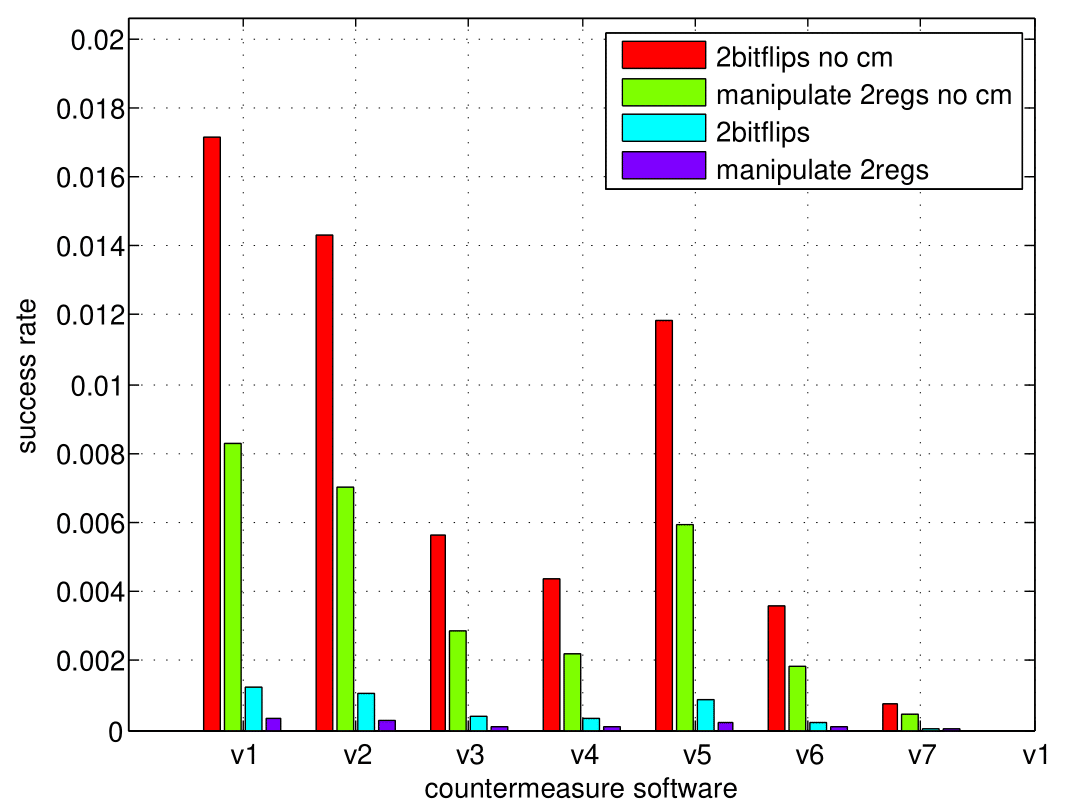
\includegraphics[width=0.99\linewidth]{Chapitre4/figures/duplication.png}
  \caption{Success rates under four fault models for seven benchmark versions with software and/without duplication countermeasures}
  \label{hwsw combine}
\end{figure}

\section{A triple-redundant countermeasure against considered fault models}

\subsection{Aim}
Neither software countermeasures, hardware countermeasures, nor their combination can fully eliminate all fault injection vulnerabilities. This limitation indicates that existing approaches are insufficient for comprehensive protection, and a new, more robust countermeasure must be designed to address all identified fault models effectively.

Among the techniques evaluated, hardware-based protections have shown superior performance in defending against the four fault models introduced in this work. Notably, they achieve this enhanced resilience without imposing significant overhead on hardware resource usage, making them a practical option for real-world deployment. Within the hardware countermeasure category, duplication and triplication architectures consistently outperform other methods, both in terms of reducing attack success rates and maintaining system stability.

Therefore, any future countermeasure design aiming for complete fault coverage should consider drawing on the structural principles of duplication and triplication. These methods provide a promising foundation for developing a more comprehensive and resilient fault-tolerant architecture.
\subsection{Presentation}

To address the four proposed vulnerability models—Bit-Flip, Manipulate Register, Two Bit-Flips, and Manipulate Two Registers—we developed a dedicated hardware-based defense mechanism. As established in our earlier analysis, software protections alone are insufficient to fully mitigate these fault models. Moreover, since no existing hardware countermeasure can comprehensively defend against all of them, we opted for a purely hardware-based solution due to its superior reliability and execution efficiency.

Our investigation also revealed that using hardware solely for fault detection is generally more effective than attempting both detection and correction. Therefore, our design prioritizes high detection accuracy, accepting a modest trade-off in correction capability and performance. The proposed solution follows a hybrid strategy that leverages the structural strengths of both duplication and triplication to form a detection-only triplication-redundant scheme. This mechanism is applied specifically to the selection register and is depicted in Figure~\ref{proposed cm}.

In this design, the output of the \texttt{SEL} register from the encoder is duplicated twice, creating two redundant copies: \texttt{cm1} and \texttt{cm2}. A comparator monitors all three register outputs, and a fault is flagged whenever any discrepancy among them is detected. The same triplication-redundant detection is applied to the \texttt{ACK} register.

\begin{figure}[t!]
  \centering
  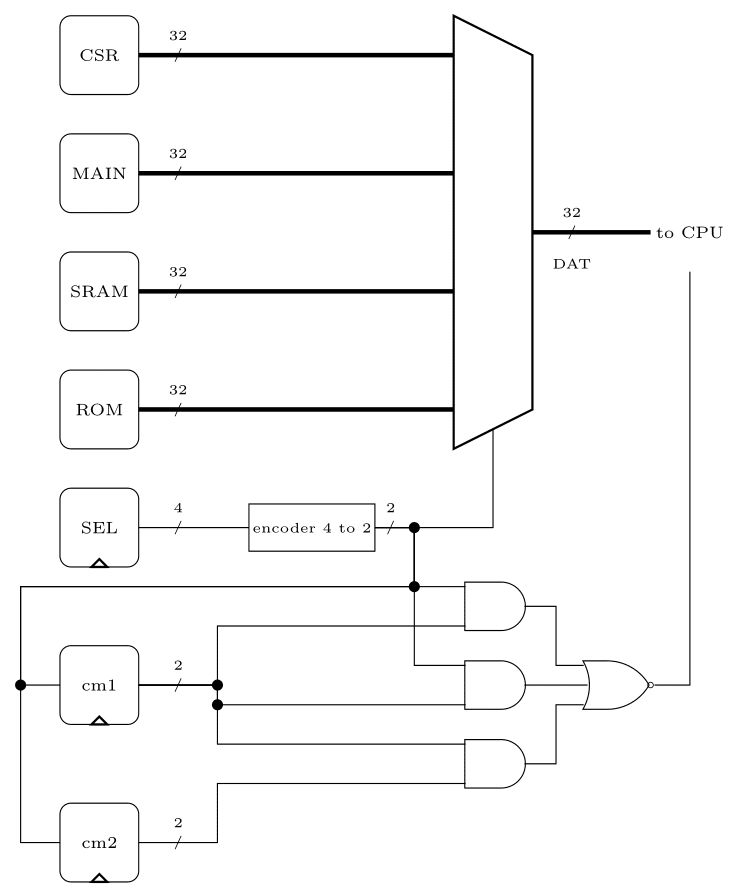
\includegraphics[width=0.9\linewidth]{Chapitre4/figures/cm tri.png}
  \caption{Our proposed countermeasure architecture on the register selection}
  \label{proposed cm}
\end{figure}

\subsection{Analysis}
 As shown in Table~\ref{tab:triplication synthesis}, compared to the baseline system without any protection, our approach increases LUT utilization by only 0.27\% and results in a negligible 0.14\% reduction in maximum clock frequency. Given that our fault model assumes no more than two simultaneously compromised registers, this two-layer redundant detection scheme effectively neutralizes all defined fault scenarios within the model's scope.

\begin{table}
    \centering
  \caption{Hardware resource overhead of Triplication-redundant countermeasure (LUT, flip-flop, frequency)}
  \label{tab:triplication synthesis}
\begin{tabular}{cccc}
\hline
countermeasure & LUT & flip-flop & frequency (MHz) \\
\hline
Unprotected & 2198 & 1793 & 70.13 \\
Triplication-redundant & 2204 & 1791 & 70.03 \\
\hline
\end{tabular}
\end{table}

To validate the robustness of our hardware-based protection, we performed a two-level verification process. First, we verified that the architecture V0 with the proposed countermeasure is resilient to hardware fault injection attacks. Second, we ensured that the architecture, when integrated with seven versions of benchmark variants designed for evaluating software-based countermeasures, also maintains its robustness. We incorporated the proposed countermeasure into all eight versions of benchmark versions under identical experimental conditions. The corresponding results are presented in Table~\ref{tab:our cm}.

\begin{table*}
  \centering
  \caption{Overall attack results on benchmarks with the proposed hardware countermeasure under four fault models}
  \label{tab:our cm}
\begin{tabular}{llrrrrr}
\hline
countermeasure                                                        & fault model      & \multicolumn{1}{c}{crash} & \multicolumn{1}{c}{detect\_hw} & \multicolumn{1}{c}{success} & \multicolumn{1}{c}{change} & \multicolumn{1}{c}{silence} \\
\hline
                                              & bit-flip          & 78                                                & 4138                                                   & 0 & 0                                                   & 698                                                 \\
                                              & manipulate reg   & 113                                               & 4805                                                   & 0 & 0                                                   & 4910                                                \\
                                              & 2 bit-flips        & 1669                                              & 46777                                                  & 0 & 0                                                  & 694                                                 \\
\multirow{-4}{*}{triplication-redundant v0} & manipulate 2 reg & 4527                                              & 140863                                                 & 0 & 0                                                  & 48362                                               \\
\hline
                                              & bit-flip          & 107                                               & 5118                                                   & 0 & 0                                                  & 865                                                 \\
                                              & manipulate reg   & 158                                               & 5937                                                   & 0 & 0                                                  & 6085                                                \\
                                              & 2 bit-flips        & 2290                                              & 57750                                                  & 0 & 0                                                  & 860                                                 \\
\multirow{-4}{*}{triplication-redundant v1} & manipulate 2 reg & 6313                                              & 173872                                                 & 0 & 0                                                  & 59935                                               \\
\hline
                                              & bit-flip          & 147                                               & 8104                                                   & 0 & 0                                                  & 1367                                                \\
                                              & manipulate reg   & 213                                               & 9412                                                   & 0 & 0                                                  & 9611                                                \\
                                              & 2 bit-flips        & 3108                                              & 91712                                                  & 0 & 0                                                  & 1360                                                \\
\multirow{-4}{*}{triplication-redundant v2} & manipulate 2 reg & 8478                                              & 276073                                                 & 0  & 0                                                 & 94673                                               \\
\hline
                                              & bit-flip          & 131                                               & 6956                                                   & 0 & 0                                                  & 1166                                                \\
                                              & manipulate reg   & 186                                               & 8080                                                   & 0 & 0                                                  & 8240                                                \\
                                              & 2 bit-flips        & 2759                                              & 78618                                                  & 0 & 0                                                  & 1153                                                \\
\multirow{-4}{*}{triplication-redundant v3} & manipulate 2 reg & 7402                                              & 236898                                                 & 0 & 0                                                  & 81104                                               \\
\hline
                                              & bit-flip          & 168                                               & 9266                                                   & 0 & 0                                                  & 1570                                                \\
                                              & manipulate reg   & 247                                               & 10759                                                  & 0 & 0                                                  & 11002                                               \\
                                              & 2 bit-flips        & 3553                                              & 104919                                                 & 0 & 0                                                  & 1568                                                \\
\multirow{-4}{*}{triplication-redundant v4} & manipulate 2 reg & 9824                                              & 315618                                                 & 0 & 0                                                  & 108430                                              \\
\hline
                                              & bit-flip          & 150                                               & 7706                                                   & 0 & 0                                                  & 1300                                                \\
                                              & manipulate reg   & 215                                               & 8949                                                   & 0 & 0                                                  & 9148                                                \\
                                              & 2 bit-flips        & 3149                                              & 87119                                                  & 0 & 0                                                  & 1292                                                \\
\multirow{-4}{*}{triplication-redundant v5} & manipulate 2 reg & 8542                                              & 262366                                                 & 0 & 0                                                  & 90100                                               \\
\hline
                                              & bit-flip          & 128                                               & 7102                                                   & 0 & 0                                                  & 1191                                                \\
                                              & manipulate reg   & 182                                               & 8251                                                   & 0 & 0                                                  & 8409                                                \\
                                              & 2 bit-flips        & 2692                                              & 80339                                                  & 0 & 0                                                  & 1179                                                \\
\multirow{-4}{*}{triplication-redundant v6} & manipulate 2 reg & 7235                                              & 242014                                                 & 0  & 0                                                 & 82779                                               \\
\hline
                                              & bit-flip          & 205                                               & 16286                                                  & 0 & 1                                                  & 2745                                                \\
                                              & manipulate reg   & 304                                               & 18935                                                  & 0 & 1                                                 & 19233                                               \\
                                              & 2 bit-flips        & 4405                                              & 185213                                                 & 0 & 2                                                  & 2742                                                \\
\multirow{-4}{*}{triplication-redundant v7} & manipulate 2 reg & 12168                                             & 556725                                                 & 0 & 19                                                 & 189555 \\                               \hline             
\end{tabular}
\end{table*}


In the final phase of our evaluation, the proposed countermeasure was deployed on the \texttt{ACK}, \texttt{SEL}, and \texttt{grant} registers. Due to time limitations, fault injection experiments were conducted only on benchmark versions V0 and V7 of the VerifyPin program. Nevertheless, these two versions are representative enough to validate the effectiveness of the countermeasure.

The results are summarized in Table~\ref{tab:complement}. After extending the countermeasure to cover the \texttt{grant} register, all observed fault injection outcomes were limited to crash, detection, or silence events. Notably, no cases of unintended memory modification were recorded. This provides strong evidence that the proposed countermeasure offers complete protection against all four fault models, irrespective of whether additional software-based protections are applied.

\begin{table}[]
  \centering
  \caption{Attack results on benchmarks with the proposed hardware countermeasure on grant register under four fault models}
  \label{tab:complement}
\begin{tabular}{llrrr}
countermeasure & fault model & \multicolumn{1}{c}{crash} & \multicolumn{1}{c}{detect\_hw} & \multicolumn{1}{c}{slience} \\
\multirow{4}{*}{triplication V0} & bitflip & 78 & 4836 & 468 \\
 & manipulate reg & 113 & 5503 & 5148 \\
 & 2 bitflip & 1825 & 57143 & 234 \\
 & manipulate 2 reg & 4979 & 175435 & 53586 \\
\multirow{4}{*}{triplication V7} & bitflip & 305 & 21808 & 2106 \\
 & manipulate reg & 451 & 24821 & 23166 \\
 & 2 bitflip & 7131 & 258225 & 1053 \\
 & manipulate 2 reg & 19818 & 792045 & 241137
\end{tabular}
\end{table}

\section{Conclusion}
In this chapter, we systematically analyzed and compared the capabilities of software and hardware countermeasures against fault injection attacks (FIAs). Software-based techniques, while offering flexibility and ease of deployment, are often limited by their vulnerability to low-level hardware faults and the constraints of the target environment. To address these shortcomings, we introduced hardware countermeasures grounded in multiplexer hardening and redundancy-based fault masking. By incorporating voting logic and path diversity into critical datapaths, these mechanisms significantly reduce the likelihood of successful fault injection.

A detailed comparison highlighted the trade-offs between software and hardware approaches in terms of coverage, cost, and implementation complexity. While software countermeasures are lightweight and adaptable, hardware solutions offer stronger resilience, especially under repeated or targeted injection scenarios. To bridge this gap, we proposed a triple-redundant countermeasure architecture tailored to the specific fault models observed in our experiments. This design ensures both error detection and recovery by introducing spatial and temporal redundancy at key signal points.

Overall, our findings demonstrate that combining lightweight software-level protections with selective, robust hardware redundancy provides a more balanced and secure defense strategy against practical fault attacks.

Based on these above findings, we offer the following recommendations for RTL-level designers seeking to design secure circuits:
\begin{enumerate}
\item Avoid using combinational logic gates for implementing multiplexers, as this can lead to multiple or no simultaneous reads, introducing vulnerabilities.
\item When hardware complexity are constrained, prioritize detection-only countermeasures and minimize their size, as they provide a lightweight yet effective defense.
\item Be aware of the interactions between software and hardware defenses: While some software defenses may reduce the success rate of hardware attacks, others may inadvertently increase their effectiveness.
\end{enumerate}